\documentclass[a4paper,12pt,twoside]{scrreprt}
% Autor der Vorlage: Klaus Rheinberger, FH Vorarlberg, 2017-02-20

% Pakete:
\usepackage[utf8]{inputenc}
\usepackage[T1]{fontenc} % Silbentrennung bei Sonderzeichen
\usepackage{graphicx} % Bilder einbinden
\usepackage{wrapfig} % Bilder positionieren
\usepackage[ngerman]{babel} % Deutsche Sprachanpassungen
\usepackage{minted} % Code Highlighting/Import
\usepackage{csquotes} % Anführungszeichen und Zitieren
\usepackage[bindingoffset=8mm]{geometry} % Bindeverlust von 8mm einbeziehen
\usepackage{caption} % Abbildungslegenden
\usepackage{xcolor} % Farbige Hervorhebungen
\usepackage{setspace} % Zeilenabstand
\usepackage[style=authoryear,citestyle=authoryear,backend=biber]{biblatex} % Literaturverweise
\usepackage[
    linktocpage=true,
    pdfauthor={Dominic Luidold},
    pdftitle={TODO}
]{hyperref} % Links -> \href{https://www.wikibooks.org}{Wikibooks home}
\usepackage[nohyperlinks]{acronym} % Abkürzungsverzeichnis

% Einstellungen:
\captionsetup{format=hang, justification=raggedright}
\addbibresource{Zotero.bib}
\setcounter{secnumdepth}{4}

% Custom Commands
\renewcommand{\listingscaption}{Quellcode}
\renewcommand\listoflistingscaption{Quellcodeverzeichnis}

% Dokumentenbeginn
\begin{document}
\onehalfspacing % Zeilenabstand 1,5

% Titelblatt:
% \newpage\mbox{}\newpage
\pagenumbering{roman}
\cleardoublepage % force output to a right page
\thispagestyle{empty}
\begin{titlepage}
    \begin{flushright}
    
\includegraphics[width=0.4\linewidth]{images/FHV_FHV-Logo.jpg}
    \end{flushright}
    \begin{flushleft}
    \section*{Vergleich der Single-page Application Frameworks Vaadin und Angular}
    \vspace{1cm}

    Bachelorarbeit II\\
    zur Erlangung des akademischen Grades
    \vspace{0.5cm}

    \textbf{Bachelor of Science in Engineering (BSc)}

    \vspace{1cm}
    Fachhochschule Vorarlberg\newline
    Informatik – Software and Information Engineering

    \vspace{0.5cm}

    Betreut von\newline
    Prof. (FH) Dipl. Inform. Thomas Feilhauer

    \vspace{0.5cm}

    Vorgelegt von\newline
    Dominic Luidold\newline
    Dornbirn, 20. Mai 2021
    \end{flushleft}
\end{titlepage}

% Widmung:
\newpage
\section*{Widmung}
\label{sec:widmung}
Zu Beginn dieser Arbeit möchte ich es mir nicht nehmen lassen, den Personen einen Dank auszusprechen, die mich bei der Umsetzung und Realisierung meiner Bachelorarbeit unterstützt haben.

\medskip

Zuerst möchte ich meinem Betreuer Thomas Feilhauer (Fachhochschule Vorarlberg) danken, der jederzeit ein offenes Ohr für Fragen, Anliegen und Unklarheiten hatte. Durch seine fachliche Kompetenz, sein Know-how und die intensive Betreuung konnte ich vieles lernen, das ich in mein fachliches sowie berufliches Leben mitnehmen kann.

\medskip

Als nächstes möchte ich meiner gesamten Familie und meinem Freund danken, denen ich während des Schreibens dieser Arbeit wahrscheinlich mehr als nur einen Nerv gekostet habe. Nur durch ihre tatkräftige Unterstützung und ihren Rückhalt konnte ich so ungestört an der Bachelorarbeit schreiben. Ohne ihr Korrekturlesen wären zudem mehr Tippfehler vorhanden als mir lieb sind und ich auf meine Tastatur schieben kann.

\medskip

Zu guter Letzt möchte ich meine Arbeit all jenen widmen, die für die Gleichbehandlung und Gleichberechtigung aller kämpfen, sich für eine Sache einsetzen, die größer als sie selbst ist und für die sie teilweise sogar ihr Leben aufs Spiel setzen. Auch 2021 braucht es weltweit immer noch laute Stimmen - Stimmen, die sich nicht unterkriegen lassen.

\bigskip

\begin{quote}
    \begin{flushright}
        \textit{\enquote{Der Fortgang der wissenschaftlichen Entwicklung ist im Endeffekt eine ständige Flucht vor dem Staunen.}}\\
        Albert Einstein
    \end{flushright}
\end{quote}

% Kurzreferat:
\newpage
\section*{Kurzreferat}
\label{sec:kurzreferat}

\subsection*{TODO}

TODO

% Abstract:
\newpage
\section*{Abstract}
\label{sec:abstract}

\subsection*{TODO}

TODO

% Geschlechtergerechte Sprache:
\newpage
\section*{Geschlechtergerechte Sprache}
\label{sec:gendern}

Der Verfasser der vorliegenden Arbeit bekennt sich zu einer geschlechtergerechten Sprachverwendung.

Um diese Arbeit sowohl geschlechtergerecht als auch -inklusive zu formulieren, wird explizit auf fix männlich oder weiblich zugeordnete Personengruppen, das sogenannte Binnen-I oder andere Schreibweisen verzichtet. Stattdessen wird auf die Schreibweise mit einem Doppelpunkt (beispielsweise \enquote{Anwender:innen}, \enquote{Entwickler:innen} etc.) gesetzt, die alle Personengruppen einschließt. Die insgesamt eventuell dadurch hervorgerufene
Irritation bei den Lesenden ist gewünscht und soll dazu beitragen, eine Bewusstheit für bestehende, diskriminierende Sprachgewohnheiten gegenüber Frauen sowie queeren Mitmenschen zu schaffen beziehungsweise zu stärken.

% Inhaltsverzeichnis:
\cleardoublepage % force output to a right page
\setcounter{tocdepth}{2}
\pdfbookmark{\contentsname}{toc}
\tableofcontents

\clearpage
\phantomsection
\addcontentsline{toc}{chapter}{Abbildungsverzeichnis}
\listoffigures

% Abkürzungsverzeichnis:
\clearpage
\phantomsection
\addcontentsline{toc}{chapter}{Abkürzungsverzeichnis}
\chapter*{Abkürzungsverzeichnis}
\begin{acronym}
  \acro{AJAX}{Asynchronous JavaScript and XML}
  \acro{API}{Application Programming Interface}
  \acro{CSS}{Cascading Style Sheets}
  \acro{DOM}{Document Object Model}
  \acro{JPA}{Jakarta Persistence}
  \acro{JSON}{JavaScript Object Notation}
  \acro{LTS}{Long Term Support}
  \acro{MPA}{Multi-page Application}
  \acro{PWA}{Progressive Web App}
  \acro{SSR}{Server-side rendering}
  \acro{SPA}{Single-page Application}
  \acro{UI}{User Interface}
  \acro{UX}{User Experience}
\end{acronym}

\cleardoublepage
\pagenumbering{arabic}
\chapter{Einleitung}
\label{chap:einleitung}
Diese Bachelorarbeit verfolgt das Ziel, einen Einblick in die \ac{SPA} Frameworks \textit{Angular}\footnote{\href{https://angular.io/}{Angular (https://angular.io)}} und \textit{Vaadin}\footnote{\href{https://vaadin.com/}{Vaadin (https://vaadin.com)}} zu geben und deren Gemeinsamkeiten, Unterschiede sowie Vor- und Nachteile zu beleuchten.

\medskip

Um ein grundlegendes Verständnis über die Thematik von \acp{SPA} zu erlangen, wird zu Beginn der Arbeit auf das Konzept einer \ac{SPA} eingegangen und die zugrundeliegende Herangehensweise mit der einer klassischen \ac{MPA} verglichen. Im weiteren Verlauf werden die unterschiedlichen Ansätze von Angular und Vaadin genauer betrachtet und eine tatsächliche Umsetzung der zuvor erläuterten Technologien mittels zweier Demo-Applikationen getestet. Am Ende dieser Arbeit wir darauf eingegangen, ob sich - anhand unterschiedlicher Kriterien und Anwendungsfälle - eine Empfehlung für eines der beiden \ac{SPA} Frameworks aussprechen lässt.

\section{Motivation}
\label{sec:motivation}
In den letzten Jahren lässt sich beobachten, dass Webapplikationen, Apps und Anwendungen allgemein verstärkt mittels des \ac{SPA}-Ansatzes umgesetzt werden und somit auf eine deutlich unterschiedlichere Herangehensweise - im Gegensatz zu klassischeren \acp{MPA} - setzen. \parencite[][]{ismail_why_2019} Für die Umsetzung einer solchen Applikation stehen eine Vielzahl von Frameworks zur Verfügung, die darüber hinaus weitere Features bieten und Entwickler:innen bei der Umsetzung unterstützen.

\newpage

Die richtige Wahl des Frameworks, der jeweiligen Technologien und der im Hintergrund agierenden Strukturen spielen eine wesentliche Rolle bei der Planung und Umsetzung eines neuen Projektes. Welches Framework sich besser eignet, lässt sich oftmals nicht auf den ersten (oder sogar zweiten) Blick feststellen. Diese Arbeit befasst sich daher genauer mit dem Konzept von \acp{SPA} und vergleicht zwei darauf aufbauende Frameworks, die mit deutlich unterschiedlichen Technologie-Stacks arbeiten und zu vergleichbaren Lösungen führen.

\section{Problemstellung}
\label{sec:problemstellung}
Die in Abschnitt \ref{sec:motivation} angesprochene Vielzahl an \ac{SPA}-Frameworks bietet grundlegend den Vorteil, dass eine große Auswahlmöglichkeit und eine gewisse Konkurrenz untereinander zu einem hohen Qualitätsstandard führt. Zudem wird dadurch sichergestellt, dass es für jedes Projekt - unabhängig von den jeweiligen Anforderungen und etwaigen Eigenheiten - eine Möglichkeit gibt, dieses mit einem der verfügbaren Frameworks umzusetzen. Auf der anderen Seite führt die stetig wachsende Anzahl an Möglichkeiten - vor allem von solchen, die auf JavaScript basieren - jedoch dazu, dass sich meist nur schwer beurteilen lässt, welches Framework und welche zugrundeliegende Technologie sich für die Umsetzung einer Applikation bestmöglich eignet.

\begin{figure}[ht]
    \centering
    
\includegraphics[scale=0.5]{images/A_JS-frameworks.png}
    \caption[Liste möglicher JavaScript-Frameworks zur Umsetzung von \acsp{SPA}]{Liste möglicher JavaScript-Frameworks zur Umsetzung von \acsp{SPA} (Quelle: \cite[][]{a_best_2020})}
    \label{fig:js-frameworks}
\end{figure}

Um eine geeignete Wahl eines Frameworks treffen zu können, sollten vorab Kriterien und Anforderungen definiert werden, die schlussendlich erfüllt werden müssen. Neben grundlegenden Funktionalitäten, die in den meisten Fällen von einer Vielzahl der Frameworks abgedeckt werden können, stellen die projektspezifischen Eigenheiten und vor allem die Auswahl der zugrundeliegenden Technologien (beispielsweise \textit{JavaScript} oder auch \textit{Java}) eine der wichtigsten Herausforderungen dar. Diese Entscheidung muss gut überlegt und abgewogen werden, da diese im weiteren Verlauf weitreichende Folgen bei der Umsetzung einer (Web-)Applikation zur Folge hat und sich ein Wechsel nach gestarteter Entwicklung nur unter großem Aufwand umsetzen lässt.

Die in Abbildung \ref{fig:js-frameworks} auf Seite \pageref{fig:js-frameworks} dargestellten Frameworks zeigen eine Auswahl an Frameworks auf, die auf \textit{JavaScript} aufbauen beziehungsweise basieren und somit primär auf dem Client, dem Browser, eingesetzt werden können. \acp{SPA} lassen sich jedoch nicht nur Frontend-seitig und vollständig mit JavaScript entwickeln (bei denen ein Großteil der Logik auf einem externen Server abläuft), sondern können auch gänzlich mittels auf Java basierenden Frameworks umgesetzt werden. Bei diesen Frameworks, zu denen Vaadin gehört, lässt sich sowohl die Logik als auch das \ac{UI} in einem einheitlichen Projekt kombinieren und entwickeln.

Da die unterschiedlichen Ansätze und Technologie-Stacks, sowohl hinter dem auf Java basierenden Vaadin als auch auf dem auf TypeScript aufbauenden Angular, gewisse Vor- und Nachteile sowie Tücken mit sich bringen, fällt die Wahl auf eines der beiden \ac{SPA}-fähigen Frameworks auf den ersten Blick nicht leicht. Hinzu kommt die Frage, welches der Frameworks weiterführende Funktionalitäten bietet, um mit geringem Aufwand beispielsweise eine \ac{PWA} umzusetzen oder anwendungsspezifische Daten lokal sowie extern persistieren zu können.

\section{Zielsetzung}
\label{sec:zielsetzung}
Die in den Abschnitten \ref{sec:motivation} und \ref{sec:problemstellung} angeführten Punkte haben aufgezeigt, dass die große Anzahl an Frameworks, mit denen \acp{SPA} umgesetzt werden können, zwar sehr positiv einzuschätzen ist, die damit verbundenen Probleme bei der Auswahl des richtigen Frameworks werden dadurch jedoch verstärkt. Aufgrund der unterschiedlichen zugrundeliegenden Technologien und einhergehenden Herangehensweisen ist eine bedachte Wahl wichtig.

\medskip

Diese Arbeit verfolgt daher das Ziel, das JavaScript/TypeScript Framework \textit{Angular} dem auf Java basierenden Framework \textit{Vaadin} gegenüberzustellen und zu vergleichen. Das Ziel ist es, mittels Literatur belegter Vergleiche einen allgemeinen Überblick über \acp{SPA} zu geben, diese klassischen Ansätzen gegenüberzustellen und zwei Demo-Applikationen zu entwickeln. Diese Webanwendungen werden dann herangezogen, um anhand von vorab definierten Kriterien feststellen zu können, ob und in wie weit Empfehlungen für eines der beiden Frameworks ausgesprochen werden können.

\medskip

Um den Fokus dieser Arbeit genauer zu definieren und einzuschränken, wird die Planung, Umsetzung sowie abschließende Beurteilung der Applikationen anhand der ausgearbeiteten Kriterien auf folgende Punkte beschränkt:
\begin{itemize}
    \item Möglichkeit zur einfachen Umsetzung einer \acf{PWA}
    \item Möglichkeit der Wiederverwendbarkeit von Komponenten, gegebenenfalls mittels \textit{Web Components}
    \item Möglichkeit Daten lokal (Browser) sowie extern (Server) zu persistieren
\end{itemize}

\chapter{Stand der Technik}
\label{chap:stand-technik}
Das folgende Kapitel gibt einen Überblick über die Funktionsweise einer \ac{SPA} und vergleicht das Konzept von \acsp{SPA} mit klassischen \acp{MPA}. Im Anschluss wird im Detail auf die Funktionsweise von Vaadin und Angular beziehungsweise deren unterschiedlichen Ansätze in Hinblick auf die Entwicklung der \acs{UI} mittels JavaScript und Java eingegangen. Im weiteren Verlauf werden die damit verbundenen Vor- und Nachteile genauer beleuchtet.

\section{Konzept einer \acs{SPA}}
\label{sec:konzept-spa}
Eine klassische \ac{MPA} basiert auf dem Konzept, dass bei jedem Aufruf eines neuen View beziehungsweise einer HTML-Seite eine Anfrage an den Server gestellt wird. Dieser verarbeitet die Anfrage und retourniert das jeweils neu zusammengestellte Resultat der Präsentations- sowie der darunterliegenden Schichten an den Client. Eine \ac{SPA} ist hingegen eine Webanwendung, bei der die Präsentationsschicht und die damit verbundene Logik vom Server entkoppelt und vollständig in den Client, sprich den Browser, ausgelagert wird. \parencite[][Seite 5ff.]{scott_spa_2015}

Die Abbildung \ref{fig:spa-overview} auf Seite \pageref{fig:spa-overview} stellt den Aufbau solch einer \ac{SPA} schematisch dar und verdeutlicht, dass die Darstellung der mittels \acs{AJAX} und XHR angeforderten Daten komplett vom Client übernommen wird. Serverseitig wird lediglich ein \textit{Controller} benötigt, welcher die übermittelten Daten in Objekte umwandeln kann, die für die Logik entsprechend verständlich sind.

\medskip

Diese Herangehensweise führt dazu, dass beim Aufrufen einer (Unter-)Seite mittels clientseitigem Routing keine komplett neue HTML-Seite geladen werden muss, sondern lediglich Teile des \acl{UI} - sogennante \textit{Views} - ausgetauscht werden. Hierfür wird das entsprechende \ac{DOM} mittels JavaScript dynamisch ausgetauscht und die benötigten Daten werden bei Bedarf asynchron mittels \acs{AJAX} und XHR vom Server geladen. \parencite[][Seite 7]{scott_spa_2015}

\begin{figure}[ht]
    \centering
    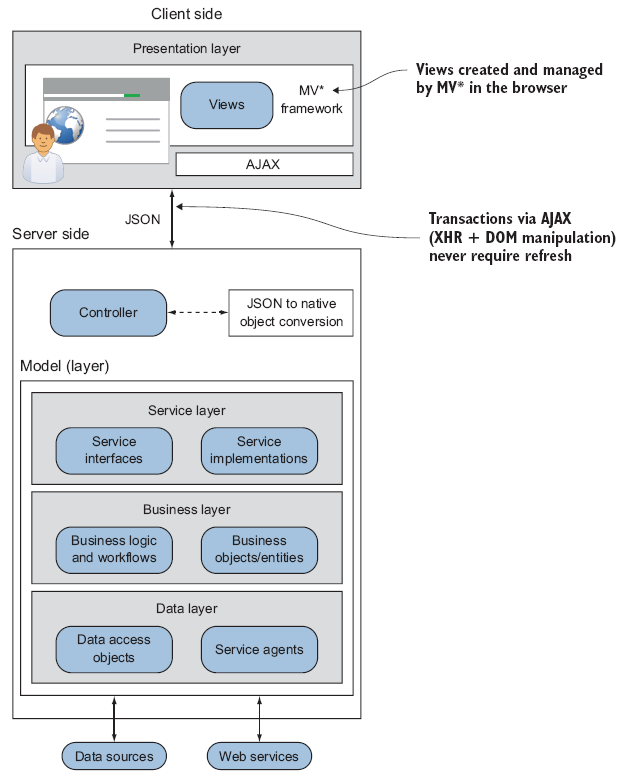
\includegraphics[scale=0.60]{images/Scott_SPA-overview.png}
    \caption[Aufbau einer \acs{SPA}]{Aufbau einer \acs{SPA}\newline(Quelle: \cite[][Seite 6]{scott_spa_2015})}
    \label{fig:spa-overview}
\end{figure}

\subsection{\acl{SSR}}
\label{subsec:ssr}
Neben der reinen Übertragung von Daten mittels \acs{JSON} (oder anderweitigen Datenformaten) kann bei \acsp{SPA} alternativ beziehungsweise erweiternd auch auf \ac{SSR} gesetzt werden. Bei diesem Ansatz werden Ausschnitte von HTML bereits auf dem Server vorbereitet und zusammen mit weiterführenden Daten an den Client geschickt. Dieser kann somit einen Teil der Antwort ohne weitere Aufbereitung darstellen, während die restlichen Daten mittels \ac{DOM}-Manipulation in die View eingebettet werden. \parencite[][Seite 7]{scott_spa_2015}

\subsection{Bestandteile einer \acs{SPA}}
\label{subsec:spa-bestandteile}
Der zugrundeliegende Aufbau einer \ac{SPA} - und der Bestandteil der Applikation, der lediglich einmal geladen wird - ist die sogenannte \textit{Shell}. Die Shell ist eine einzelne HTML-Datei, welche vom Browser vollständig geladen wird und in den meisten Fällen lediglich minimale Strukturen (ein Navigationsmenü, statische Inhalte etc.) sowie einen leeren \texttt{DIV} Tag enthält, wie Abbildung \ref{fig:spa-shell} auf Seite \pageref{fig:spa-overview} zeigt. Genutzt wird diese als Ausgangspunkt für alle weiteren Views, die unabhängig von der Shell agieren und dynamisch geladen werden. \parencite[][Seite 8]{scott_spa_2015}

\begin{figure}[ht]
    \centering
    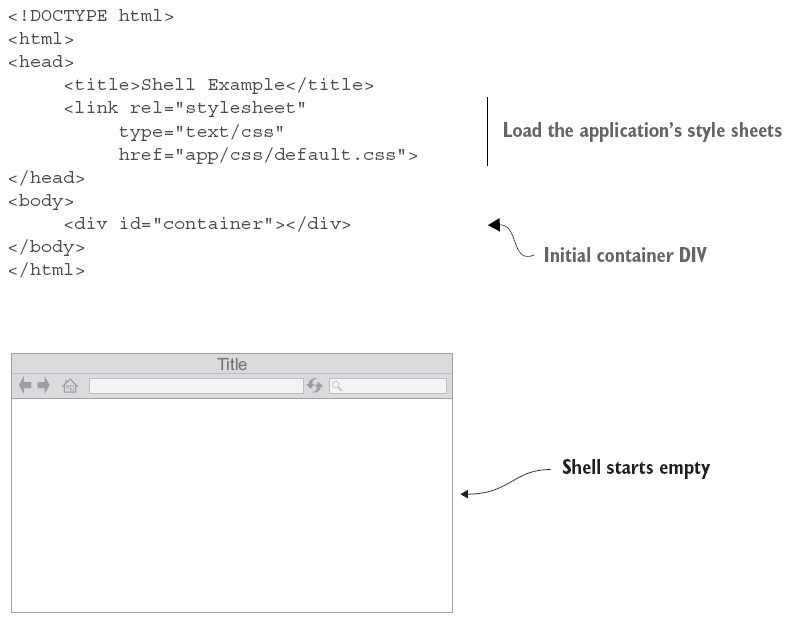
\includegraphics[scale=0.45]{images/Scott_SPA-shell.png}
    \caption[\acs{SPA} Shell]{\acs{SPA} Shell\newline(Quelle: \cite[][Seite 8]{scott_spa_2015})}
    \label{fig:spa-shell}
\end{figure}

Voneinander getrennt sichtbare Bereiche der Anwendung können im weiteren Verlauf ebenfalls mit \texttt{DIV} Tags abgegrenzt werden und sind dem in der Shell definierten \texttt{DIV} Container untergeordnet. Dies ermöglicht sowohl eine logische als auch inhaltliche Gruppierung und das gezielte Austauschen bestimmter Bereiche, sogenannter \textit{Regions}. \parencite[][Seite 9]{scott_spa_2015}

\medskip

Die einzeln dargestellten Views, welche dynamisch ausgetauscht werden können, stellen keine vollständigen HTML-Seiten dar, sondern bilden lediglich gezielt definierte Ausschnitte. Diese Ausschnitte werden bei jedem Navigationsvorgang innerhalb der Website durch das entsprechend eingesetzte Framework ausgetauscht und erfordern kein erneutes Laden der Website. \parencite[][Seite 10f.]{scott_spa_2015}

\section{Vorteile einer \acs{SPA} gegenüber einer \acs{MPA}}
\label{sec:vorteile-spa-mpa}
Der Einsatz und die Entwicklung einer \ac{SPA} bietet sowohl Vorteile für Entwickler:innen als auch Anwender:innen gegenüber der Nutzung einer klassischen \ac{MPA}.

Der bereits mehrfach angesprochene Vorgang, lediglich bestimmte Teile beziehungsweise Views der Webanwendung auszutauschen, erhöht die Benutzbarkeit sowie die \ac{UX} laut Mikowski und Powell deutlich. Da keine komplett neue (Unter-)Seite geladen werden muss, entfällt das Aufscheinen einer - abhängig von der Internet- und Servergeschwindigkeit - kurz sichtbaren, weißen Übergangsseite während des Ladeprozesses. Dem:Der Benutzer:in kann stattdessen beispielsweise ein dynamisch dargestellter Fortschrittsbalken dargestellt werden, der sich bei vorhandener Ladezeit laufend aktualisiert. \parencite[][Seite 20]{mikowski_single_2013}

Scott hebt hervor, dass die Aufteilung in eine entkoppelte Präsentationsschicht auf dem Client dazu führt, dass diese unabhängig von der Logik auf dem Server gewartet und aktualisiert werden kann. Während bei klassischen \acsp{MPA} stellenweise HTML, JavaScript etc. mit serverseitigem Code (beispielsweise \textit{PHP}, \textit{JavaServer Pages}, ...) vermischt werden, kann bei \acsp{SPA} zudem eine gewisse Differenzierung und Abtrennung von HTML, \ac{CSS} und JavaScript im Frontend erzielt werden, was die Wartbarkeit ebenfalls erhöht. \parencite[][Seite 13]{scott_spa_2015}

\newpage

Sowohl Mikowski und Powell als auch Scott gehen des Weiteren darauf ein, dass die Datenübertragung und Verarbeitung bei einer \ac{SPA} effizienter und schneller stattfinden kann, als bei einer \ac{MPA}. Die Programmlogik zur Darstellung und dynamischen Entscheidungsfindung befindet sich beim Client (weshalb dieser Operationen schnell durchführen kann), während der Server lediglich Validierung, Authentifizierung und Datenspeicherung durchführt. \parencite[][Seite 20]{mikowski_single_2013} Zudem sind Transaktionen zwischen Client und Server nach dem Initialen Aufruf der Applikation schneller, da lediglich Daten in einem vorab definierten Datenformat asynchron übertragen und keine kompletten HTML-Seiten samt JavaScript und \ac{CSS} ausgetauscht werden müssen. \parencite[][Seite 13]{scott_spa_2015}

\section{Funktionsweise von Vaadin}
\label{sec:funktionsweise-angular-vaadin}
Sowohl Angular als auch Vaadin sind beides Frameworks, die das Entwickeln von \acp{SPA} unterstützen und ermöglichen. Der gewählte Ansatz, die zugrundeliegenden Technologien und die jeweiligen Herangehensweisen unterscheiden sich stellenweise jedoch deutlich voneinander.

Der nachfolgende Abschnitt befasst sich daher im Detail mit der Funktionsweise und den Konzepten von Vaadin sowohl aus dem Blickwinkel von Entwickler:innen als auch Anwender:innen. Wo sinnvoll, wird ein direkter Vergleich zu Angular gezogen und darauf eingegangen, wie die beiden Frameworks Probleme unterschiedlich handhaben und lösen.

\subsection{Ansätze von Vaadin}
\label{sub-sec:vaadin-ansaetze}
Vaadin ist ein Framework beziehungsweise eine Plattform, mit der Webapplikationen sowohl komplett in Java, vollständig mit TypeScript und HTML als auch in einer Kombination beider entwickelt und umgesetzt werden können. Die beiden Ansätze sind dabei in zwei verschiedene Frameworks aufgeteilt, um - je nach Einsatzzweck - diese entsprechend einzusetzen:

\begin{itemize}
    \item \textbf{Vaadin Flow} ist ein Framework, mit dem Webapplikationen in Java umgesetzt werden können. Technologien wie beispielsweise HTML oder JavaScript werden bei der Entwicklung der \acs{UI} nicht benötigt, der gesamte Programmcode basiert auf einer einheitlichen Programmiersprache. Die gesamte Anwendung selbst läuft auf einem Server, während das Framework den Applikationszustand sowie die Client-Server-Kommunikation übernimmt.  \parencite[][]{vaadin_ltd_vaadin_nodate}
    \item \textbf{Vaadin Fusion} ist ein Framework, bei dem TypeScript für das Frontend auf dem Client und Java für das Backend auf dem Server eingesetzt wird. Mit Fusion können clientseitig reaktive Webapplikationen entwickelt werden, die typsichere Java Endpunkte aufrufen. Vorgefertigte Komponenten erleichtern hierbei das Entwickeln der \acs{UI}, während eigene Elemente mittels voller Kontrolle über das \ac{DOM} umgesetzt werden können. \parencite[][]{vaadin_ltd_vaadin_nodate-1}
\end{itemize}

Diese Arbeit befasst sich nachfolgend primär mit \textit{Vaadin Flow}, um eine alternative Herangehensweise aufzuzeigen, wie eine \ac{SPA} komplett auf dem Server und mittels Java entwickelt werden kann. Durch diesen Fokus kann im weiteren Verlauf ein tiefergehenderer Vergleich der Funktionalitäten und Konzepte von Vaadin und Angular bewerkstelligt werden, der bei spezifischen Punkten konkret auf die Unterschiede der beiden Technologien eingeht.

\subsection{Frontend und Backend in Java}
\label{sub-sec:frontend-backend-java}
Vaadin selbst schreibt, dass sich das Arbeiten mit HTML, \ac{CSS} und JavaScript für reine Java-Entwickler sowohl als herausfordernd als auch als zeitintensiv darstellt. \parencite[][Framework - Introduction - Overview]{vaadin_ltd_documentation_nodate}

Vaadin Flow bietet daher die Möglichkeit, mit einer vollständig in Java geschriebenen Applikation - die auf einem Server ausfgeführt wird - jeweils die Anwendungslogik sowie das \acl{UI} umzusetzen. Die Vielzahl von sogenannten \textit{Components}, welche Vaadin von Haus aus mitliefert und einzelnen Bestandteilen wie beispielsweise einem Button oder ähnlichem entspricht, unterstützen Entwickler:innen dabei, bei Bedarf ohne HTML oder JavaScript auszukommen. Die Components steuern dabei das zugrundeliegende JavaScript im Hintergrund über die Framework-eigene \textit{Java API} beziehungsweise die \textit{Java Component API}. Der Quellcode \ref{code:vaadin-ui-java-sample} auf Seite \pageref{code:vaadin-ui-java-sample} stellt einen stark vereinfachten Ausschnitt von Components dar, die so im Client bereits entsprechend dargestellt werden. \parencite[][Framework - Introduction - Overview]{vaadin_ltd_documentation_nodate}

\begin{listing}[ht]
    \inputminted[fontsize=\footnotesize,linenos]{java}{code/Vaadin_Java-UI-sample.java}
    \caption[Beispiel einer einfachen \acs{UI} mittels der \textit{Java API}]{Beispiel einer einfachen \acs{UI} mittels der \textit{Java API}\newline(Quelle: \cite[][]{vaadin_ltd_overview_2021})}
    \label{code:vaadin-ui-java-sample}
\end{listing}

Während mit Vaadin Flow hauptsächlich in Java, und somit auf dem Server, entwickelt wird, bietet das Framework dennoch die Möglichkeit, auf Browser \acsp{API}, spezifische Web Components sowie auf das \ac{DOM} zuzugreifen.

Als Vorteil stellt sich zudem heraus, dass die Anbindung des Frontends an ein Backend in den meisten Fällen mit Vaadin Flow bereits komplett vorhanden ist und nicht separat mit auf REST basierender Kommunikation umgesetzt werden muss. Dadurch kann die \acs{UI} und die dafür benötigten Daten direkt über Java verknüpft und auch aktualisiert werden. Hierbei unterstützen mitgelieferte \textit{Events} und \textit{Event Listener} die Entwicklung und Benutzbarkeit, indem Änderungen auf dem Client automatisch auch auf dem Server - und umgekehrt - abgebildet werden. \parencite[][]{vaadin_ltd_overview_2021-2}

\subsection{Kommunikation zwischen Client und Server}
\label{sub-sec:kommunikation-client-server}
Bei einer \ac{SPA} spielt die Kommunikation des Clients (dem JavaScript/Type-Script Frontend) und dem Server (dem Backend) eine sehr wichtige Rolle. Im Gegensatz zu \acp{MPA}, bei denen die Daten bereits auf dem Server verarbeitet, eingebettet und als Ganzes übertragen werden, werden bei \acsp{SPA} diese erst bei Bedarf und im Nachhinein geladen. Die Art und Weise, wie dieser Vorgang umgesetzt wird, unterscheidet sich bei Vaadin Flow und Angular jedoch deutlich voneinander.

\subsubsection{Automatische Kommunikation von Vaadin}
\label{sub-sub-sec:kommunikation-herangehensweise-vaadin}
Da sowohl die Persitenzschicht, die Applikationslogik als auch das \acl{UI} bei Vaadin Flow mittels Java umgesetzt werden können, ergibt sich der Vorteil, dass die Kommunikation zwischen Client und Server vom Framework selbst übernommen wird und hierbei unter anderem auf das bereits angesprochene \textit{Two-way data binding} setzt. Die Nutzung von Vaadin-eigenen Components bietet des Weiteren die Möglichkeit, das \ac{DOM} im Webbrowser selbst zu steuern, während eine Repräsentation desselben \ac{DOM} serverseitig in Java gehalten wird. Änderungen, die auf dem Client durchgeführt werden, werden automatisch synchronisiert. \parencite[][Framework - Introduction - Core Concepts]{vaadin_ltd_documentation_nodate}

\medskip

Artur Signell, CTO der Vaadin Ltd., erklärt währenddessen in einem Foren-Beitrag vom Juni 2018, dass genauere Informationen zur tatsächlich Umsetzung der automatisch vorgenommen Kommunikation nicht nach außen kommuniziert werden, da die Umsetzung davon als rein internes Implementierungsdetail gehandhabt wird. \parencite[][]{signell_explanation_2018}

\medskip

Mittels den Entwicklertools, die in gängigen Webbrowsern zur Verfügung stehen, kann sich - abseits der nicht vorhandenen Dokumentation - jedoch ein kurzes Bild davon gemacht werden, wie die Kommunikation grundsätzlich funktioniert. Die Abbildung \ref{fig:vaadin-json-communication} auf Seite \pageref{fig:vaadin-json-communication} zeigt die vom Client an den Server geschickte Anfrage, die durch das Befüllen eines Vaadin \texttt{TextField} (einem HTML - \texttt{INPUT} Element) ausgelöst wird. Für die Kommunikation wird \acs{JSON} eingesetzt, welches die in das \texttt{INPUT} Element eingefüllten Daten mit gängiger HTTP-Kommunikation an den Server schickt, auf die schlussendlich mittels Java-typischer Notation zugegriffen werden kann.

\begin{figure}[ht]
    \centering
    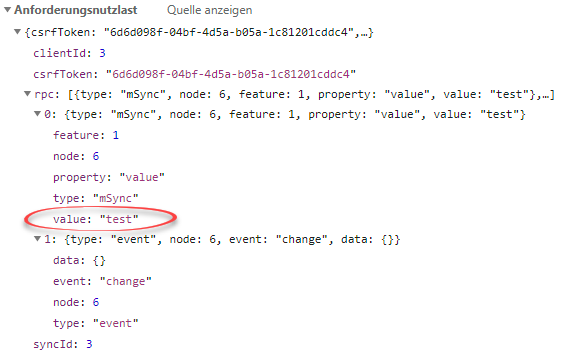
\includegraphics[scale=0.75]{images/Luidold_Vaadin-HTTP-communication.png}
    \caption[Automatisch erzeugte Kommunikation von Vaadin Flow]{Automatisch erzeugte Kommunikation von Vaadin Flow\newline(Quelle: eigene Abbildung)}
    \label{fig:vaadin-json-communication}
\end{figure}

\newpage

\subsubsection{Anpassbare Kommunikation bei Angular}
\label{sub-sub-sec:kommunikation-herangehensweise-angular}
Im Vergleich zur automatischen Kommunikation, die Vaadin Flow von Haus aus bietet, unterstützt Angular Entwickler:innen zwar beim Datenaustausch mit einem Server, die konkrete Umsetzung muss jedoch deutlich eigenständiger programmiert werden.

\medskip

Der von Angular entwickelte \texttt{HttpClient} Service - der über das \path{@angular/common/http} Package bezogen werden kann - stellt eine entsprechende API zur Verfügung, mit der typisierte \texttt{Response} Objekte angefordert werden können, eine vereinheitlichte Fehlerbehandlung ermöglicht wird sowie das Abfangen und Bearbeiten von \texttt{Request} und \texttt{Response} Objekten erlaubt. \parencite[][]{google_llc_communicating_nodate}

\medskip

Der Einsatz der angesprochenen API kann bei Angular grundsätzlich im gesamten Projekt erfolgen, Wilken empfiehlt jedoch, die Nutzung von der tatsächlichen Logik zu abstrahieren und dafür einen eigenständigen Service zu erstellen. Der \texttt{HttpClient}, welcher zur Kommunikation mit einem Server (und gegebenenfalls in einem eigenständigen Service) verwendet wird, unterstützt HTTP Request-Methoden wie beispielsweise \texttt{GET}, \texttt{POST}, \texttt{PUT} und \texttt{DELETE}, die bei einem entsprechenden Aufruf ein \texttt{Observable} als Antwort liefern. Mit diesem kann in weiterer Folge in der Applikation gearbeitet und auf die Daten zugegriffen werden. \parencite[][Seite 142-144.]{wilken_angular_2018}

\medskip

Der Quellcode \ref{code:angular-sample-httpclient-service} auf Seite \pageref{code:angular-sample-httpclient-service} zeigt einen exemplarischen Service, der mittels \texttt{HTTP GET} eine Anfrage an den Server beziehungsweise einen API Endpunkt stellt und ein Array des Typs \texttt{Sample} als Antwort zurückliefert.

\begin{listing}[ht]
    \renewcommand{\fcolorbox}[4][]{#4}
    \inputminted[fontsize=\footnotesize,linenos]{js}{code/Luidold_HttpClient-Service.ts}
    \caption[Exemplarische Nutzung des \texttt{HttpClient} in einem Service]{Exemplarische Nutzung des \texttt{HttpClient} in einem Service}
    \label{code:angular-sample-httpclient-service}
\end{listing}

Der Quellcode \ref{code:angular-sample-data-function} auf Seite \pageref{code:angular-sample-data-function} zeigt in Folge die Nutzung der gerade eben demonstrierten Funktion, bei der die Daten mittels \texttt{subscribe()} abgefragt werden können und entsprechend zugewiesen werden, sobald diese zur Verfügung stehen.

\begin{listing}[ht]
    \renewcommand{\fcolorbox}[4][]{#4}
    \inputminted[fontsize=\footnotesize,linenos]{js}{code/Luidold_Load-function.ts}
    \caption[Beispielhafte Nutzung der \texttt{getSampleData} Funktion]{Beispielhafte Nutzung der \texttt{getSampleData} Funktion}
    \label{code:angular-sample-data-function}
\end{listing}

Verglichen mit der im Abschnitt \ref{sub-sub-sec:kommunikation-herangehensweise-vaadin} auf Seite \pageref{sub-sub-sec:kommunikation-herangehensweise-vaadin} beschriebenen Herangehensweise von Vaadin unterscheidet sich Angular deutlich. Wilken merkt an, dass die Nutzung des \texttt{HttpClient} der am häufigsten verwendete Ansatz bei Angular darstellt. Um eine Kommunikation mit einem Server herzustellen, können laut ihm jedoch auch, beziehungsweise zusätzlich, diverse andere Protokolle und Technologien genutzt werden. \parencite[][]{wilken_angular_2018}

\subsection{Vaadin Components und deren Grundlage}
\label{sub-sec:vaadin-components}
\textit{Vaadin Components} sind von Vaadin entwickelte \enquote{\acs{UI}-Module}, die zur einfachen Entwicklung von gängigen \acl{UI} Bestandteilen genutzt werden können. Diese sind bereits im Vaadin Framework enthalten, können im Zuge der Nutzung der Web Components Technologien jedoch unabhängig von Vaadin selbst und somit in allen gängigen Applikationen sowie Webbrowsern genutzt werden. \parencite[][Seite 2ff.]{vaadin_ltd_vaadin_nodate-2}

Die Abbildung \ref{fig:vaadin-components-overview} auf Seite \pageref{fig:vaadin-components-overview} zeigt hierbei eine Auswahl von Vaadin Components, die häufig in Webapplikationen genutzt werden und entsprechend für das Framework umgesetzt wurden.

\begin{figure}[ht]
    \centering
    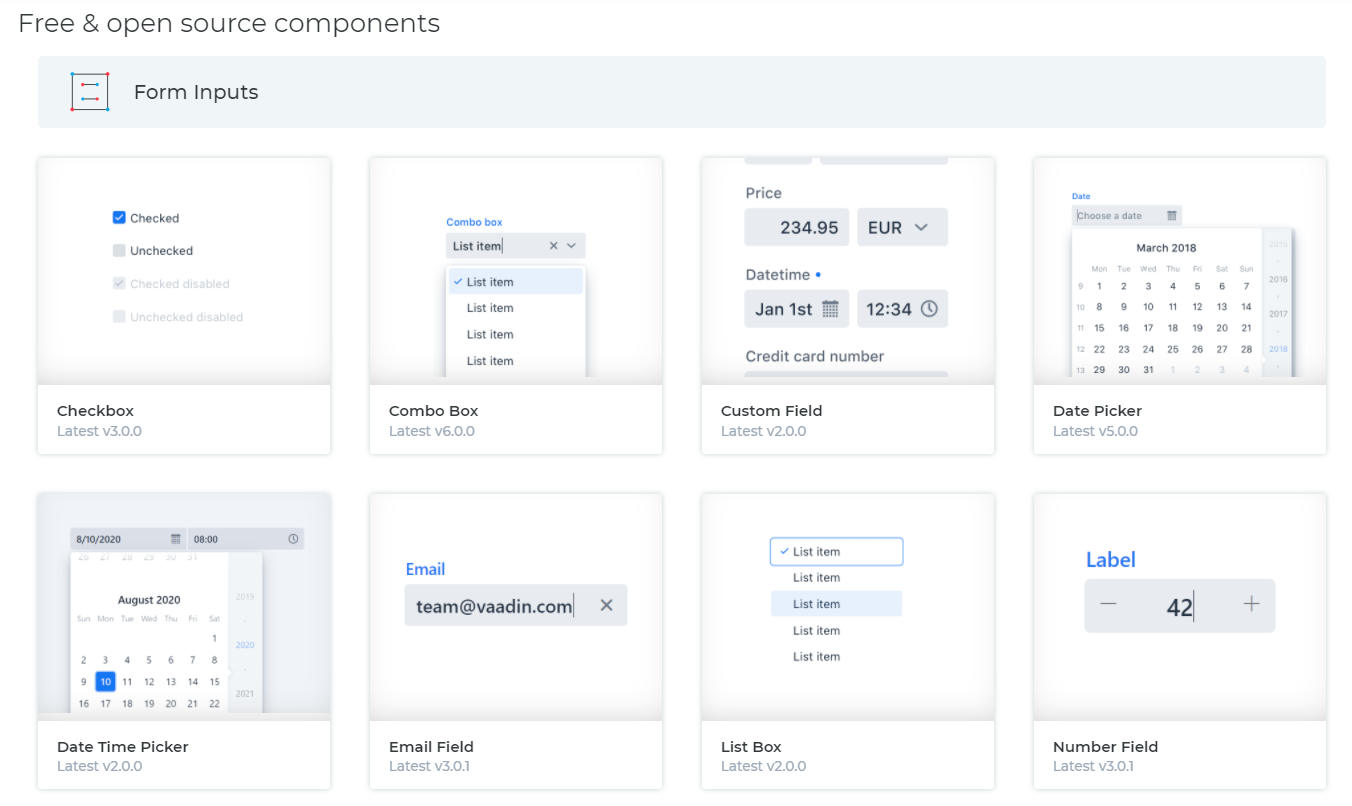
\includegraphics[scale=0.38]{images/Vaadin_Components-overview.png}
    \caption[Auswahl von Open Source Vaadin Components]{Auswahl von Open Source Vaadin Components\newline(Quelle: \cite[][]{vaadin_ltd_mobile_nodate})}
    \label{fig:vaadin-components-overview}
\end{figure}

Die Technologien, auf die sich Vaadin bei der Implementierung und Umsetzung der Components stützt, bauen auf diversen Konzepten auf, zu denen unter anderem \textit{Custom elements}, \textit{Shadow \ac{DOM}} sowie \textit{HTML templates} gehören. Diese werden dazu genutzt, um mittels JavaScript spezifische Klassen für die gewünschten, neuen Web Components zu erstellen, diese entsprechend zu registrieren und mittels Template-Funktionalität die neu erstellten Objekte schlussendlich zu definieren. \parencite[][]{mozilla_contributors_web_2021}

\medskip

Der Quellcode \ref{code:mozilla-sample-web-component} auf Seite \pageref{code:mozilla-sample-web-component} zeigt beispielhaft auf, wie der grundlegende Aufbau eines eigens umgesetzten Web Components aussieht. Vaadin nutzt diesen Aufbau sowie die zugrundeliegende Herangehensweise für die Umsetzung der vorhergehend aufgezeigten \textit{Vaadin Components}. \parencite[vgl.][]{vaadin_ltd_vaadin-text-fieldjs_2021} Aufgrund des Fokus dieser Arbeit wird im weiteren Verlauf jedoch nicht näher auf die zugrundeliegende Struktur von Web Components eingegangen.

\begin{listing}[ht]
    \inputminted[fontsize=\footnotesize,linenos]{js}{code/Mozilla_Web-Component-sample.js}
    \caption[Beispiel für den grundlegenden Aufbau eines eigenen Web Components]{Beispiel für den grundlegenden Aufbau eines eigenen Web Components (Quelle: \cite[][]{mozilla_contributors_using_2021})}
    \label{code:mozilla-sample-web-component}
\end{listing}

Die Nutzung der Vaadin Components lässt sich sowohl eigenständig mit anderen Frameworks als auch direkt in Vaadin selbst mittels der sogenannten \textit{Java API} umsetzen. Jede Komponente besitzt beim Einsatz von Java entsprechende Objekt-Typen und dazugehörige Attribute, bei der Verwendung von HTML stehen Tags mit ähnlicher Funktionalität zur Verfügung. \parencite[][]{vaadin_ltd_mobile_nodate}

\medskip

Quellcode \ref{code:vaadin-textfield} auf Seite \pageref{code:vaadin-textfield} ermöglicht einen Einblick, wie ein \textit{Text Field} Component mittels Vaadins Java API genutzt werden kann. Die deklarierten und initialisierten \texttt{TextField} Objekte können, in Java typischer Weise, an beliebiger Stelle genutzt werden. Weiterführende beziehungsweise benötigte Funktionalitäten können im Anschluss über das Zuweisen und Setzen von spezifischen Attributen erzielt werden, die das Verhalten des Textfeldes beeinflussen und vorgeben.

\begin{listing}[ht]
    \inputminted[fontsize=\footnotesize,linenos]{java}{code/Vaadin_Text-Field_sample.java}
    \caption[Mögliche Umsetzungen des Vaadin \textit{Text Field}]{Mögliche Umsetzungen des Vaadin \textit{Text Field}\newline(Quelle: \cite[][Basic text field]{vaadin_ltd_java_nodate})}
    \label{code:vaadin-textfield}
\end{listing}

Abbildung \ref{fig:vaadin-textfield-output} auf Seite \pageref{fig:vaadin-textfield-output} bezieht sich maßgeblich auf Quellcode \ref{code:vaadin-textfield}, da die dargestellten Textfelder jene sind, die mittels der aufgezeigten \texttt{TextField} Objekte erzeugt wurden und mittels gesetzter Attribute unterschiedliche Ausgangspunkte liefern.

\begin{figure}[ht]
    \centering
    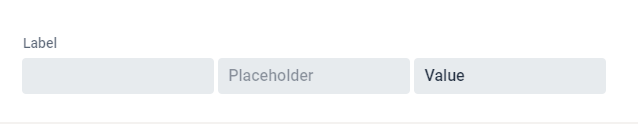
\includegraphics[scale=0.7]{images/Vaadin_Text-Field-output.png}
    \caption[Erzeugter Output von Quellcode \ref{code:vaadin-textfield}]{Erzeugter Output von Quellcode \ref{code:vaadin-textfield}\newline(Quelle: \cite[][Basic text field]{vaadin_ltd_java_nodate})}
    \label{fig:vaadin-textfield-output}
\end{figure}

\subsection{Routing und Navigation}
\label{sub-sec:routing-navigation}
Wilken schreibt, dass die meisten Webapplikationen die Funktionalität benötigen, während der Nutzung zwischen verschiedenen Seiten und Unterseiten navigieren zu können. \acp{MPA} laden beim Aufruf einer Seite die hinterlegten HTML, \ac{CSS} und JavaScript Dateien von einem Webserver und nutzen dafür die angegebene URL. \acp{SPA} hingegen laden Daten asynchron und bei Bedarf und wechseln lediglich sogenannte Views und keine kompletten Seiten. Die Navigation innerhalb einer \ac{SPA} muss entsprechend anderweitig vorgenommen werden, wobei hier sowohl JavaScript an sich als auch das verwendete Framework eine wichtige Rolle spielt. \parencite[][Seite 159f.]{wilken_angular_2018}

\subsubsection{Routing bei Vaadin}
\label{sub-sub-sec:routing-herangehensweise-vaadin}
Vaadin bietet die Möglichkeit, mittels der \texttt{@Route} Annotation alle Components (sowohl Vaadin Components als auch eigene) über eine spezifische URL ansprechbar zu machen und diese somit aufrufen zu können. Quellcode \ref{code:route-annotation-vaadin} auf Seite    \pageref{code:route-annotation-vaadin} stellt beispielhaft dar, wie eine selbst entwickelte Komponente im Browser über die URL \path{http://example.com/some/path} angesteuert werden kann. \parencite[][Using the @Route Annotation]{vaadin_ltd_overview_2021-1}

\begin{listing}[ht]
    \inputminted[fontsize=\footnotesize,linenos]{java}{code/Vaadin_Route-annotation.java}
    \caption[Beispielhafte Nutzung der \texttt{@Route} Annotation]{Beispielhafte Nutzung der \texttt{@Route} Annotation\newline(Quelle: \cite[][Using the @Route Annotation]{vaadin_ltd_overview_2021-1})}
    \label{code:route-annotation-vaadin}
\end{listing}

Mittels verschiedener Events, die während der Nutzung der Webapplikation und der darin auftretenden Navigation ausgelöst werden, entsteht ein sogenannter \textit{Navigation Lifecycle}. Dieser kann dafür genutzt werden, um zusätzliche Funktionalitäten anzubieten. UI Komponenten implementieren dafür entsprechende \texttt{Listener}, welche auf zugehörigen \texttt{Observer} Interfaces aufbauen. Mit dem Navigation Lifecycle und einem \texttt{BeforeLeaveEvent} kann beispielsweise eine Abfrage im \acl{UI} erstellt werden, die Nutzer:innen bestätigen lässt, dass das Verlassen der Website womöglich zum Verlust von Daten führt. \parencite[][]{vaadin_ltd_navigation_2021}

\newpage

URL Parameter (sowohl solche, die Teil der URL selbst sind als auch Query Parameter) können mittels dem \texttt{HasUrlParameter} Interface abgefragt und im weiteren Verlauf genutzt werden. Wie Quellcode \ref{code:url-params-vaadin} auf Seite \pageref{code:url-params-vaadin} zeigt, kann über die \texttt{setParameter} Methode auf Teile der URL zugegriffen werden, die mittels Generics direkt in der Methode verankert sind. \parencite[][]{vaadin_ltd_typed_2021} Query Parameter lassen sich währenddessen mit dem \texttt{BeforeEvent} ebenfalls in derselben Methode abfragen. \parencite[][]{vaadin_ltd_query_2021}

\begin{listing}[ht]
    \inputminted[fontsize=\footnotesize,linenos]{java}{code/Luidold_Vaadin-URL-params.java}
    \caption[Zugriff auf URL Parameter bei Vaadin]{Zugriff auf URL Parameter bei Vaadin}
    \label{code:url-params-vaadin}
\end{listing}

\smallskip

Um die Navigation zwischen verschiedenen Routen zu ermöglichen, bietet Vaadin - neben dem händischen Abändern der URL im Browser - verschiedene Ansätze:

\begin{itemize}
    \item Mittels der \texttt{RouterLink} Komponente können Links erstellt werden, welche die angegebene Route als Ziel haben (\texttt{menu.add(new RouterLink("Home", HomeView.class));}). \parencite[][Using the RouterLink Component]{vaadin_ltd_navigating_2021}
    \item Gewöhnliche HTML Anker Tags können genutzt werden, um zwischen verschiedenen Routen zu navigieren (\texttt{<a href="company" [...]}). Diese verursachen jedoch ein Neuladen der gesamten Seite. Wenn der zusätzliche Ladeprozess der Seite verhindert werden soll, kann das Vaadin-eigene \texttt{router-link} Attribut zusätzlich angehängt werden. \parencite[][Using Standard href Links]{vaadin_ltd_navigating_2021}
    \item Serverseitig kann mittels \texttt{UI.navigate(/* Route name */)} der Wechsel zu einer neuen Route ausgelöst werden. \parencite[][Server-side Navigation]{vaadin_ltd_navigating_2021}
\end{itemize}

\subsubsection{Routing bei Angular}
\label{sub-sub-sec:routing-herangehensweise-angular}
Um bei Angular eine vergleichbare Routing und Navigation Funktionalität zu erzielen, wird das \path{@angular/router} Package benötigt, welches in das Projekt eingebunden werden muss. Anders als bei Vaadin können bei Angular Routen an zentraler Stelle definiert werden, bei denen angegeben wird, welche TypeScript Komponente für die Abhandlung zuständig ist, wie Quellcode \ref{code:angular-route-definition} auf Seite \pageref{code:angular-route-definition} zeigt. \parencite[][]{google_llc_angular_nodate}

\begin{listing}[ht]
    \inputminted[fontsize=\footnotesize,linenos]{js}{code/Angular_Routes-definition.js}
    \caption[Definition von Routen bei Angular]{Definition von Routen bei Angular\newline(Quelle: \cite[][]{google_llc_angular_nodate})}
    \label{code:angular-route-definition}
\end{listing}

Vom Prinzip her ähnlich bietet Angular ebenfalls die Möglichkeit, auf die in der URL enthaltenen Parameter zuzugreifen und in der Präsentations- sowie Applikationslogik zu verwenden. Hierfür wird das \texttt{ActivatedRoute} Objekt dem Konstruktor einer Komponente übergeben, welches sowohl den Zugriff auf die Query Parameter (\texttt{ActivatedRoute\#queryParams}) als auch Parameter, die Bestandteil der URL sind (\texttt{ActivatedRoute\#paramMap}), ermöglicht. Zudem stehen allgemeine Informationen zur Route selbst zur Verfügung. \parencite[][]{google_llc_angular_nodate}

\medskip

Links innerhalb der \acs{UI} werden - vergleichbar mit Vaadin - ebenso mit HTML Anker Tags und einem eigens dafür vorgesehenen Attribut erzeugt, beinhalten im Zuge der entsprechenden Darstellungsoptionen jedoch noch weitere Funktionalitäten. Quellcode \ref{code:angular-route-linking} auf Seite \pageref{code:angular-route-linking} stellt diesen Ansatz dar und beinhaltet zudem in Zeile 19 das benötigte \texttt{<router-outlet>} Element, welches die ausgewählten und geladenen Routen im Browser darstellt. \parencite[][]{google_llc_angular_nodate}

\begin{listing}[ht]
    \inputminted[fontsize=\footnotesize,linenos]{html}{code/Angular_Routing-tags.html}
    \caption[Verlinken von Routen innerhalb von Angular]{Verlinken von Routen innerhalb von Angular\newline(Quelle: \cite[][]{google_llc_angular_nodate})}
    \label{code:angular-route-linking}
\end{listing}

\chapter{Methodik und Vorgehensweise}
\label{chap:methodik-vorgehensweise}
Die in Kapitel \ref{chap:stand-technik} ab Seite \pageref{chap:stand-technik} behandelten Punkte befassen sich mit den grundlegenden Konzepten einer \ac{SPA} und den spezifischen Funktionalitäten sowie Herangehensweisen, auf denen Vaadin basiert. Wo sinnvoll, wurde zudem ein Vergleich zu Angular gezogen.

In den folgenden Kapiteln fokussiert sich diese Arbeit nun auf die Planung, Umsetzung und Beurteilung von zwei Demo-Applikationen, die auf denselben User Stories basieren, jedoch sowohl mit Vaadin als auch Angular umgesetzt werden. Ziel ist es, diese Webapplikationen entlang vorab definierter Kriterien zu entwickeln, um schlussendlich eine Bewertung durchführen zu können.

\section{Kriterien}
\label{sec:kriterien}
Die Kriterien, anhand derer sich die Umsetzung und Beurteilung richten werden, wurden bereits in der Einleitung im Abschnitt \ref{sec:zielsetzung} ab Seite \pageref{sec:zielsetzung} kurz aufgegriffen. Da diese jedoch noch nicht im Detail behandelt wurden, folgt in den nächsten Absätzen eine entsprechend genauere Darstellung.

\subsubsection*{Umsetzung als \acl{PWA}}
\label{sub-sec:kriterien-pwa}
Die Demo-Applikationen sollen in mehrerer Hinsicht als moderne Webapplikation genutzt werden können. Dazu gehört, neben der standardmäßigen Nutzung mittels gängiger Webbrowser auf dem Desktop, die Nutzung als \ac{PWA}, die vor allem für Smartphones optimiert und ausgelegt ist und sich ähnlich wie eine App verhält.

Bei der Umsetzung und Bewertung wird daher darauf eingegangen, in wie weit sich die Webanwendungen mit den von Vaadin und Angular zur Verfügung gestellten Mitteln als \acp{PWA} umsetzen lassen und welche Funktionalitäten schlussendlich zur Verfügung stehen.

\subsubsection*{Einsatz und Entwicklung von wiederverwendbaren Komponenten}
\label{sub-sec:kriterien-web-components}
In Abschnitt \ref{sub-sec:vaadin-components} wurde bereits auf die Vaadin eigenen \textit{Vaadin Components} eingegangen. Da die Wiederverwendbarkeit in der Entwicklung eine große Rolle spielt, und auch auf \acs{UI}-Komponenten zutrifft, sollen mehrfach verwendete Bestandteile der Demo-Applikationen wiederverwendbar, und wo sinnvoll, mit Web Components umgesetzt werden.

Bei der Umsetzung und Bewertung wird daher darauf eingegangen, in welchem Ausmaß die Frameworks die Umsetzung dieses Vorhabens - zusätzlich zu den gegebenen Browserstandards - unterstützen und ob sie den Entwicklungsprozess dabei erleichtern.

\subsubsection*{Lokale und serverseitige Datenanbindung/-haltung}
\label{sub-sec:kriterien-datenanbindung}
\acp{SPA}, beziehungsweise Anwendungen allgemein, leben von den Daten, die sie verarbeiten und mit denen Nutzer:innen interagieren können. Gerade im Zuge der Umsetzung der Demo-Applikationen als \ac{PWA} stellt sich die Frage, wie Angular und Vaadin eine Datenanbindung und Datenhaltung lokal (sprich auf dem jeweiligen Endgerät) sowie auf einem Server ermöglichen.

Bei der Umsetzung und Bewertung wird daher darauf eingegangen, welche Möglichkeiten sich bieten, bei den entwickelten Anwendungen Daten sowohl lokal zu speichern (um beispielsweise eine Offline-Fähigkeit zu ermöglichen) und wie man diese an eine externe Datenbank auf einem Server anbinden kann.

\section{Vorgehensweise}
\label{sec:vorgehensweise}
Damit die Demo-Applikationen die eben genannten Kriterien beide gleichermaßen beinhalten und umsetzen, und somit bewertet werden können, werden diese in User Stories eingebettet. Die User Stories orientieren sich dabei jedoch an keinem vollständigen Applikations-Konzept, sondern zeigen verschiedene Anwendungsfälle auf, die in einem realen Umfeld ein Bewertungskriterium für die Auswahl eines Frameworks spielen können.

\subsection{User Stories}
\label{sub-sec:user-stories}
Nachfolgend sind zwei User Stories aufgelistet, die im Detail erklären, welche Funktionalitäten die Vaadin und Angular Demo-Applikation beinhalten sollen und die genannten Kriterien einfließen lassen.

\subsubsection*{User Story 1: Echtzeit Eingangskontrolle}
\label{sub-sub-sec:user-story-1}

\paragraph*{Beschreibung:} Als Veranstalter:in einer Organisation möchte ich kommende und gehende Besucher:innen bei allen Ein-/Ausgängen in Echtzeit erfassen, sodass diese den Veranstaltungsort nur in kontrollierter Weise betreten können.

\paragraph*{Akzeptanzkriterien:}

\begin{itemize}
    \item Besucher:innen können aus einer vorhandenen Teilnehmer:innenliste ausgewählt werden, um festzulegen, ob sie sich innerhalb oder außerhalb vom Veranstaltungsort befinden.
    \item Wird der Status eine:r Besucher:in aktualisiert, wird diese Änderung automatisch auf allen Instanzen sichtbar, ohne dass man diese manuell neu laden muss. Dies entspricht entspricht der Multi-Nutzer:innen-Fähigkeit.
    \item Die Anwendung wird sowohl auf Computern als auch im mobilen Einsatz auf einem gängigen Smartphone unterstützt.
    \item Wenn keine Internetverbindung vorhanden ist, ist zumindest der zuletzt verfügbare Stand der Besucher:innenliste aufrufbar.
\end{itemize}

\subsubsection*{User Story 2: Fotoverwaltung}
\label{sub-sub-sec:user-story-2}

\paragraph*{Beschreibung:} Als Nutzer:in möchte ich meine Fotos hochladen können, sodass diese an einem zentralen Ort gespeichert sind und man jederzeit darauf zugreifen kann.

\paragraph*{Akzeptanzkriterien:}

\begin{itemize}
    \item Nutzer:innen können Fotos von ihrem Computer oder Smartphone auswählen und hochladen, damit diese in einer zentralen Galerie angesehen werden können.
    \item Wenn Fotos von einem anderen Client hochgeladen wurden, kann man diese mit dem aktuellen Gerät ebenso ansehen, ohne dieser erneut hochzuladen oder synchronisieren zu müssen.
    \item Wenn keine Internetverbindung vorhanden ist, werden Fotos lokal gespeichert und können hochgeladen werden, sobald wieder eine Verbindung zur Verfügung steht.
\end{itemize}

\chapter{Umsetzung}
\label{chap:umsetzung}
Damit das Ziel dieser Arbeit - einen Vergleich zwischen den beiden \ac{SPA} Frameworks Vaadin und Angular herzustellen - erreicht werden kann, wurden zwei Demo-Applikationen nach den in Kapitel \ref{chap:methodik-vorgehensweise} ab Seite \pageref{chap:methodik-vorgehensweise} aufgezeigten Methoden und Herangehensweisen entwickelt.

Bevor auf die erzielten Ergebnisse eingegangen wird, folgt in diesem Kapitel eine kurze Erläuterung dazu, wie die zwei Webanwendungen gestartet beziehungsweise verwendet werden können und wie deren Entwicklung und Umsetzung abgelaufen ist. Zudem wird kurz auf einige (technische) Hürden eingegangen, die währenddessen aufgetreten sind.

Der Quellcode der beiden Anwendungen ist der physischen Abgabe als Kopie beigelegt und zusätzlich jederzeit auf GitHub abrufbar: \url{https://github.com/DominicLuidold/Bachelor-Thesis-II}

\section{Vaadin Demo-Applikation}
\label{sec:vaadin-demo}
Als erste der beiden Applikationen wurde die Vaadin Demo umgesetzt und \textit{\nameref{sub-sub-sec:user-story-1}} sowie \textit{\nameref{sub-sub-sec:user-story-2}} dafür abgeschlossen. Die Entwicklung wurde bewusst aufgeteilt, sodass währenddessen ein Fokus auf das jeweilige Framework und die entsprechenden Technologien gelegt werden konnte und kein kontinuierliches Umdenken erforderlich war.

\medskip

Zur Umsetzung der Vaadin Demo-Applikation kommt die Version \texttt{19.0.2} zum Einsatz, die zum Stand des Entwicklungsbeginns Anfang März 2021 die aktuellste Version darstellt. In  Kapitel \ref{chap:stand-technik} ab Seite \pageref{chap:stand-technik} wurden stellenweise Auszüge aus der Dokumentation zu Vaadin \texttt{18.x} verwendet, diese behalten jedoch weiterhin ihre Gültigkeit und haben sich nur marginal verändert.

\subsection{Starten und Verwenden der Vaadin Demo}
\label{sub-sec:starten-verwenden-vaadin}
Vaadin Flow unterstützt sowohl für die aktuelle \ac{LTS} Version \texttt{14.x} als auch für Version \texttt{19.x} den Einsatz von Java \texttt{8}, \texttt{11} und \texttt{16}. Im Zuge der Umsetzung der Vaadin Demo wird auf Java \texttt{11} gesetzt, weshalb diese Version auf dem ausführenden System installiert sein muss.

Zusätzlich zu einer vorhandenen Java Umgebung wird \textit{Apache Maven}\footnote{\href{https://maven.apache.org/}{Apache Maven (https://maven.apache.org)}} benötigt, welches alle projektspezifischen Abhängigkeiten lädt und verwaltet. Abgesehen von einem gängigen Webbrowser müssen keine zusätzlichen Tools/etc. heruntergeladen werden.

\medskip

Die Vaadin Webanwendung kann verhältnismäßig einfach gestartet werden und unterstützt dabei zwei verschiedene Modi (für beide muss man vorab in das entsprechende Anwendungsverzeichnis navigieren):

\begin{itemize}
    \item \textbf{Development Mode:} Im Anwendungsverzeichnis \path{vaadin-demo-app/} muss lediglich der Befehl \underline{\texttt{mvn}} in einem Terminal eingegeben werden. Daraufhin werden alle benötigten Abhängigkeiten automatisch geladen und nach kurzer Zeit ist die Anwendung unter \url{http://localhost:8080} aufrufbar.
    \item \textbf{Production Mode:} Die Vorgehensweise ist ähnlich zum Development Mode, statt dem direkten Ausführen der Anwendung im jeweiligen Terminal wird nach der Eingabe von \underline{\texttt{mvn clean package -Pproduction}} eine \texttt{.jar} Datei im Ordner \path{target/} erstellt. Diese kann im weiteren Verlauf dafür genutzt werden, die Webanwendung auf einem beliebigen System auszuführen und bereitzustellen.
\end{itemize}

\subsection{Entwickeln mit Vaadin}
\label{sub-sec:entwickeln-vaadin}
Das Entwickeln einer Vaadin Flow Applikation benötigt nur wenige technische Voraussetzungen, die in Abschnitt \ref{sub-sec:starten-verwenden-vaadin} auf Seite \pageref{sub-sec:starten-verwenden-vaadin} bereits aufgezeigt wurden. Vaadin selbst erleichtert den Start zudem mittels einer eigenen Website\footnote{\href{https://vaadin.com/start}{Get Started | Vaadin (https://vaadin.com/start)}}, auf der verschiedene \textit{Hello World}-Beispiele heruntergeladen werden können. Bei Bedarf können zudem erste Konfigurationsschritte im Browser getätigt und das daraus resultierende Projekt als Start für die Entwicklung genutzt werden.

\medskip

Die für diese Arbeit entwickelte Vaadin Demo-Applikation setzt neben den bereits genannten Komponenten auch auf Spring Boot, welches beim Erstellen einer neuen Vaadin Flow Anwendung standardmäßig mitgeliefert wird. Spring Boot hat sich während der Umsetzung als wichtiges Hilfsmittel erwiesen, da entsprechend zur Verfügung stehende Annotations und eine einfache Integration mit dem ORM-Framework \textit{Hibernate} die Entwicklung beschleunigt und den benötigten Konfigurationsaufwand deutlich minimiert haben. Die \textit{Live Reload}\footnote{\href{https://vaadin.com/docs/latest/guide/live-reload}{Live Reload (https://vaadin.com/docs/latest/guide/live-reload)}} Funktionalität hat es zudem ermöglicht, Änderungen am Java Quellcode vorzunehmen, während der Applikationsserver gestartet ist. Diese Änderungen werden durch den optimierten \enquote{Restart} deutlich schneller im Browser dargestellt, verglichen mit dem händischen Stoppen und erneutem Starten der Anwendung.

\medskip

Das Arbeiten mit der von Vaadin veröffentlichten Dokumentation selbst hat in den meisten Fällen gut funktioniert. Verglichen mit anderen Frameworks oder Tools hat sich jedoch bereits früh bemerkbar gemacht, dass Vaadin deutlich weniger beziehungsweise eingeschränkter eingesetzt wird. Neben der offiziellen Dokumentation und einigen hilfreichen Foreneinträgen bei Vaadin selbst, finden sich nur wenige Lösungsansätze auf den gängigen Entwickler-Plattformen oder bei der Nutzung einer der gängigen Suchmaschinen. Dieser Umstand hat sich vor allem dann als Nachteil herausgestellt, wenn die verfügbaren Ansätze entweder unvollständig oder nicht sehr detailreich waren und das Verständnis für die entsprechende Herangehensweise von Vaadin noch nicht gänzlich vorhanden ist.

\medskip

Abseits der angebrachten Punkte  stellt sich das Arbeiten mit Vaadin Flow vor allem für Entwickler:innen, die bereits mit Java gearbeitet haben, jedoch als gewohnt dar und funktioniert gut. HTML oder JavaScript Kenntnisse werden keine benötigt und die \textit{Vaadin Components} beziehungsweise eigene Komponenten lassen sich meist mit wenigen Zeilen \ac{CSS} an die jeweiligen Bedürfnisse anpassen.

\section{Angular Demo-Applikation}
\label{sec:angular-demo}
Nach der abgeschlossenen Entwicklung der Vaadin Demo wurde der Fokus auf die Entwicklung der Angular Demo und dem dazugehörigen \textit{Node.js}\footnote{\href{https://https://nodejs.org/}{Node.js (https://nodejs.org)}} Backend gelegt, die ebenfalls \textit{\nameref{sub-sub-sec:user-story-1}} sowie \textit{\nameref{sub-sub-sec:user-story-2}} beinhalten.

Um die Angular Webanwendung verwenden zu können, bedarf es - im Vergleich zur Vaadin Umsetzung - zwei verschiedener und weitestgehend unabhängiger Projekte beziehungsweise Applikationen. Auf der einen Seite die Applikation, die im Client dargestellt und angewandt werden kann und auf der anderen Seite jene, die auf einem Server läuft und Daten verarbeitet, bereitstellt sowie zentral persistiert.

\medskip

Zur Umsetzung der Angular Demo-Applikation kommen Angular \texttt{11.2} für die Frontend-Entwicklung und Node.js \texttt{14.16} mit Express \texttt{4.17} im Backend zum Einsatz. Sowohl das Frontend als auch das Backend werden mittels TypeScript (in der Version \texttt{4.x}) entwickelt und für den schlussendlichen Betrieb zu JavaScript kompiliert. Die verwendeten Versionen entsprechen zum Stand des Entwicklungsbeginns Ende März 2021 jeweils den aktuellsten Versionen beziehungsweise bei Node.js der aktuellen \ac{LTS} Version.

\subsection{Starten und Verwenden der Angular Demo}
\label{sub-sec:starten-verwenden-angular}
Da die Angular Demo in zwei separate Projekte aufgeteilt ist, müssen diese auch jeweils eigenständig gestartet werden. Als Voraussetzung dafür wird in beiden Fällen lediglich eine vorhandene Node.js Installation benötigt, welche \textit{npm} mitliefert und damit die Verwaltung der projektspezifischen Abhängigkeiten übernimmt.

\medskip

Im Regelfall sollte zuerst das Backend gestartet werden, bevor im Anschluss die Angular Webanwendung selbst in Betrieb genommen wird. Um das Backend zu starten, müssen folgende Schritte durchgeführt werden:

\clearpage

\begin{itemize}
    \item \textbf{Abhängigkeiten installieren:} Im Verzeichnis \path{angular-backend/} müssen die benötigten Abhängigkeiten mittels \underline{\texttt{npm install}} installiert werden.
    \item \textbf{Backend starten:} Anschließend muss, ebenfalls im Anwendungsverzeichnis, der Node.js Server mit dem Ausführen des Befehls \underline{\texttt{npm start}} gestartet werden. Nach kurzer Zeit steht das Backend unter \url{http://localhost:8181} zur Verfügung.
\end{itemize}

Die Angular Demo kann mit etwas mehr Aufwand, aber dennoch verhältnismäßig einfach, gestartet werden und unterstützt dabei wieder zwei verschiedenen Modi (hierbei ist zu beachten, dass die \ac{PWA} Funktionalität lediglich im \textit{Production Mode} zur Verfügung steht):

\begin{itemize}
    \item \textbf{Development Mode:} Im Anwendungsverzeichnis \path{angular-demo-app/} müssen zuerst die Abhängigkeiten mittels \underline{\texttt{npm install}} installiert werden. Anschließend kann die Angular Demo über das Ausführen der Befehle \underline{\texttt{npm install -g @angular/cli}} und \underline{\texttt{ng serve -o}} gestartet werden und ist nach kurzer Zeit unter \url{http://localhost:4200} aufrufbar.
    \item \textbf{Production Mode:} Nach dem Laden der Abhängigkeiten (siehe Development Mode) muss die Anwendung mit dem Befehl \underline{\texttt{ng build -{}-prod}} für den Production Mode vorbereitet werden. Sobald der Vorgang abgeschlossen ist, stehen die fertigen Projektdateien im Anwendungsverzeichnis im Ordner \path{dist/angular-demo-app/} zur Verfügung. \newline
    Diese Dateien können jedoch nicht direkt aufgerufen werden, sondern müssen dem Browser von einem Webserver zur Verfügung gestellt werden. Mit \underline{\texttt{npm install -g http-server}} kann ein kleiner HTTP-Server installiert werden, der anschließend über ein Terminal mit den Befehlen \underline{\texttt{cd dist/angular-demo-app/}} und  \underline{\texttt{http-server -o -p 8282}} gestartet werden kann. Die Anwendung steht nach kurzer Zeit unter \url{http://localhost:8282} zum Aufruf bereit und enthält, im Vergleich zum Development Mode, die \ac{PWA} Funktionalität.
\end{itemize}

Zu beachten ist, dass die Angular Demo standardmäßig nur auf dem Gerät funktionsfähig ist, auf dem auch das Node.js Backend gestartet wurde. Um das zu ändern, muss im Verzeichnis \path{angular-demo-app/src/environments/} in der Datei \texttt{environment.ts} die IP Adresse individuell angepasst werden. Im \textit{Development Mode} werden die Änderungen automatisch übernommen, im \textit{Production Mode} müssen die oben angeführten Schritte erneut vorgenommen werden.

\subsection{Entwickeln mit Angular und Node.js}
\label{sub-sec:entwickeln-angular}
Ähnlich wie bei der Entwicklung mit Java und Vaadin, erfordert das Arbeiten mit den (Web-)Technologien - auf denen sowohl die Angular Demo-Applikation und das dazugehörige Backend basieren - nur wenige technische Voraussetzungen (siehe dazu Abschnitt \ref{sub-sec:starten-verwenden-angular} ab Seite \pageref{sub-sec:starten-verwenden-angular}).

Während es für einen Node.js Server unzählige Anleitungen und Beispiele im Internet gibt, unterstützt Angular den Entwicklungsstart und auch die weiterführende Umsetzung mit der \textit{Angular CLI}\footnote{\href{https://angular.io/cli}{Angular CLI (https://angular.io/cli)}}. Sowohl das Erstellen eines \textit{Hello World} Projekts als auch das Generieren von gängigen Komponenten lässt sich damit einfach handhaben und wurde während der Entwicklung aktiv eingesetzt.

\medskip

Im Vergleich zur Vaadin Demo hat sich der Programmieraufwand hierbei leicht erhöht, da neben der eigentlichen Anwendung selbst auch ein dazugehöriges Backend entwickelt werden musste. Da beide Anwendungen auf Type- Script, und somit JavaScript, basieren und die Herangehensweise ähnlich ist, hat dieser Umstand die Entwicklung jedoch nicht spürbar negativ beeinflusst. Als wichtiger Punkt kommt hinzu, dass die zur Verfügung stehende Dokumentation ausreichend ist und vor allem der große Vorteil besteht, dass sowohl Angular als auch Node.js mit einem \textit{Express}\footnote{\href{https://expressjs.com/}{Express (https://expressjs.com)}} Server sehr weit verbreitet sind. Entsprechende Suchen in den gängigen Suchmaschinen führen zu unzähligen Tutorials, Antworten auf gängige Fragen und Beispielen, die bei der Entwicklung extrem hilfreich sein können.

\medskip

Sofern technische \enquote{Hürden} während der Entwicklung aufgetreten sind, hatten diese primär mit der Umsetzung der \ac{PWA} Funktionalität zu tun. Die von Angular bereitgestellte \ac{PWA} Implementierung lässt sich nur in dem in Abschnitt \ref{sub-sec:starten-verwenden-angular} ab Seite \pageref{sub-sec:starten-verwenden-angular} dargelegten \textit{Production Mode} testen. Vorgenommene Änderungen können daher nicht wie gewohnt direkt begutachtet werden, sondern müssen zuerst den immer gleichen Prozess durchlaufen. Zudem haben die Browser die Website des öfteren gecached, sobald die \ac{PWA} genutzt oder installiert wurde. Dadurch war nicht immer direkt ersichtlich, ob nun die aktuelle Version dargestellt wird und ob diese bereits aktualisiert wurde.

\medskip

Der Umstieg auf einen Mix zwischen HTML, \ac{CSS} und JavaScript/TypeScript hat sich bei der Umsetzung am deutlichsten bemerkbar gemacht und ist auch einer der offensichtlichen Punkte, in denen sich Vaadin und Angular unterscheiden. Sowohl der deutlich größere Projektumfang als auch die veränderten Programmierparadigmen erfordern eine gewisse Einarbeitungszeit, was sich während der Entwicklung an machen Stellen als Vorteil, an anderen Stellen aber auch als Nachteil erwiesen hat. Für Entwickler:innen, die bisher noch wenig mit diesen Technologien gearbeitet haben, ist der Einstig jedoch gut möglich und wahrscheinlich etwas leichter, verglichen mit Vaadin und dem objektorientierten Ansatz von Java.

\chapter{Ergebnisse}
\label{chap:ergebnisse}
In den vorhergehenden Kapiteln wurde auf den aktuellen \textit{\nameref{chap:stand-technik}} eingegangen, die \textit{\nameref{chap:methodik-vorgehensweise}} der zu dieser Arbeit gehörenden Entwicklung beleuchtet und anschließend auf die \textit{\nameref{chap:umsetzung}} eingegangen. Neben den Erfahrungen, die sich primär auf die Entwicklung selbst beziehen und in Kapitel \ref{chap:umsetzung} ab Seite \pageref{chap:umsetzung} bereits beschrieben wurden, spielen vor allem aber die tatsächlich erzielten Ergebnisse der Vaadin und Angular Applikationen eine entscheidende Rolle.

In den nachfolgenden Abschnitten wird daher detailliert darauf eingegangen, wie die schlussendlichen Resultate ausgefallen sind und wie diese technisch umgesetzt wurden. Wo sinnvoll, wird zusätzlich die Anwendung aus der Sicht von Nutzer:innen beleuchtet und die Unterschiede sowie Ähnlichkeiten der beiden Demo-Applikationen aufgegriffen.

\section{Die \acsp{SPA} im \enquote{äußerlichen} Vergleich}
\label{sec:applikationen-design-vergleich}
Die Demo-Applikationen wurden so entwickelt, dass sowohl die Vaadin als auch die Angular Umsetzung jeweils dieselben Funktionalitäten (soweit möglich) aufweisen und den Nutzer:innen anbieten. Das zugrundeliegende Aussehen der Anwendungen war von dieser Anforderung jedoch ausgenommen, weshalb zwei stellenweise sehr unterschiedliche Resultate entstanden sind.

\medskip

Bei der Entwicklung der Angular Webanwendung kam die von Angular selbst entwickelte \textit{Material UI component library}\footnote{\href{https://material.angular.io/}{Angular Material (https://material.angular.io)}} zum Einsatz. Diese stellt diverse \textit{Components} - wie beispielsweise Tabellen, Buttons, \enquote{Snackbars} etc. - zur Verfügung, die anschließend in der Anwendung verwendet und beliebig angepasst werden können. Die Abbildung \ref{fig:results-angular-ec-snackbar} auf Seite \pageref{fig:results-angular-ec-snackbar} zeigt die eben genannten Components in der Angular Demo im Einsatz. Der Stil von Angular Material ist dabei am Material Design von Google\footnote{\href{https://material.io/}{Material Design (https://material.io)}} angelehnt und ähnelt dem Aussehen des Betriebssystems Android sowie gewissen, dafür verfügbaren Apps. Die Verwendung der verschiedenen Komponenten gestaltet sich als relativ einfach, bezogen auf das Anpassen des jeweiligen Aussehens und Verhaltens bei unterschiedlichen Geräte- und Displaygrößen.

\begin{figure}[ht]
    \centering
    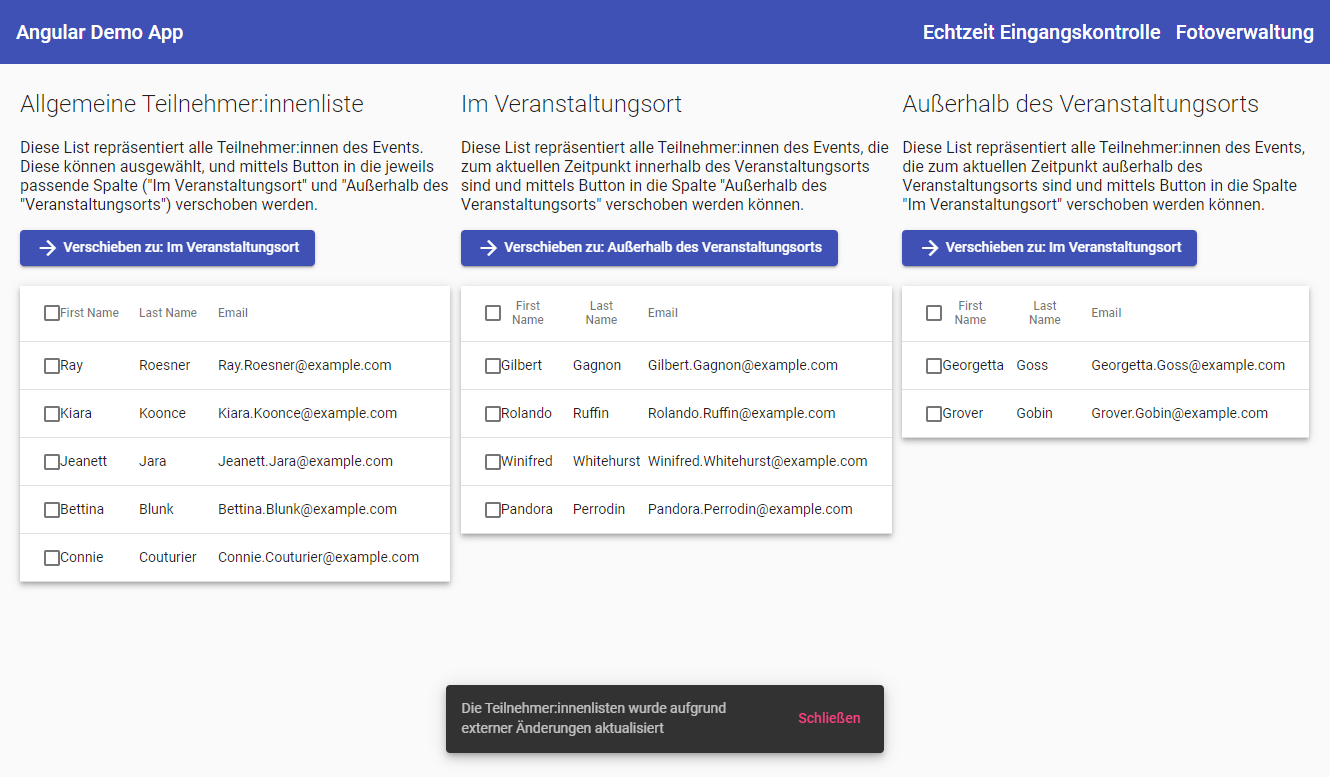
\includegraphics[scale=0.4]{images/Luidold_Results-Angular-EntranceControl-Snackbar.png}
    \caption[Funktionalität \textit{Echtzeit Eingangskontrolle}, umgesetzt mit Angular]{Funktionalität \textit{Echtzeit Eingangskontrolle}, umgesetzt mit Angular}
    \label{fig:results-angular-ec-snackbar}
\end{figure}

Die Vaadin Applikation baut währenddessen auf den in Abschnitt \ref{sub-sec:vaadin-components} ab Seite \pageref{sub-sec:vaadin-components} beschriebenen \textit{Vaadin Components} auf, welche beim sogenannten \enquote{Styling} vergleichbar mit den Komponenten von Angular sind. Der von Vaadin standardmäßig zur Verfügung gestellte Stil verfolgt dabei ein deutlich anderes Design-Konzept, wie Abbildung \ref{fig:results-vaadin-ec-snackbar} auf Seite \pageref{fig:results-vaadin-ec-snackbar} aufzeigt.

\begin{figure}[ht]
    \centering
    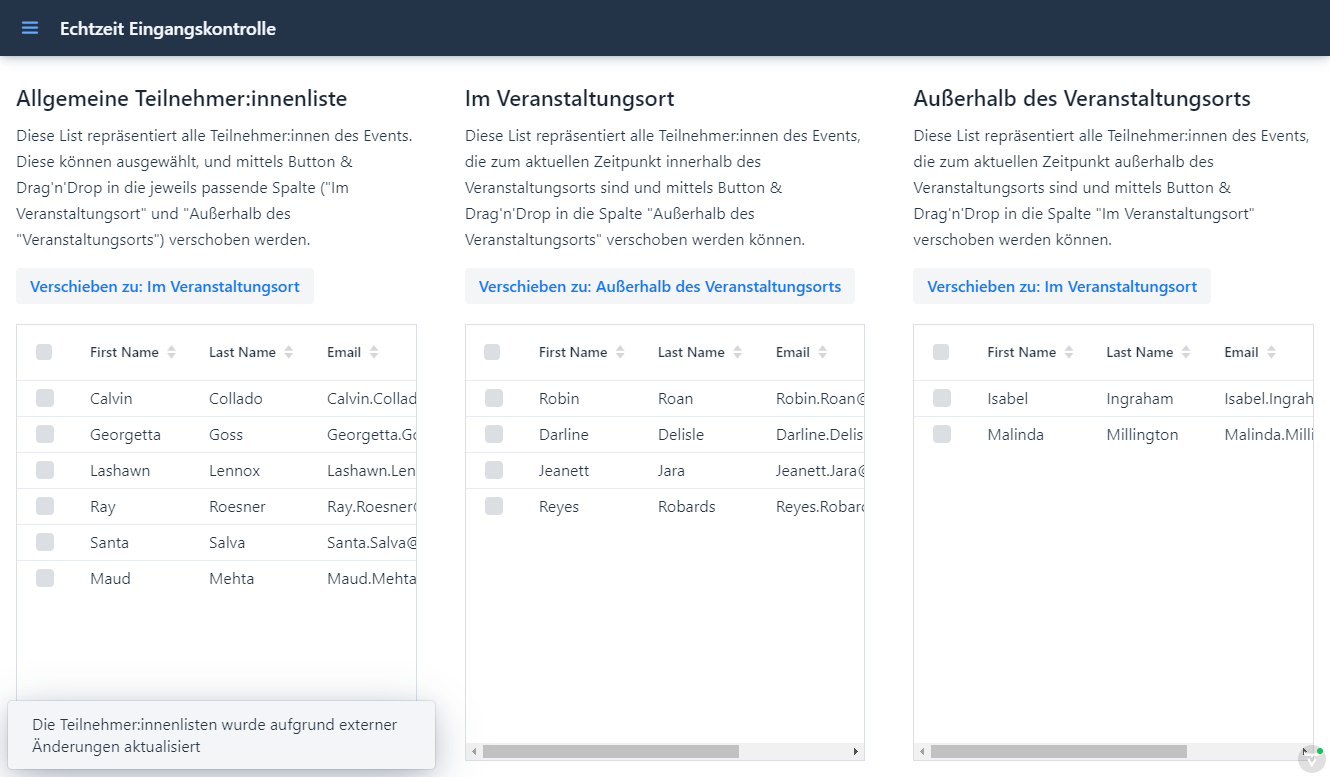
\includegraphics[scale=0.4]{images/Luidold_Results-Vaadin-EntranceControl-Snackbar.png}
    \caption[Funktionalität \textit{Echtzeit Eingangskontrolle}, umgesetzt mit Vaadin]{Funktionalität \textit{Echtzeit Eingangskontrolle}, umgesetzt mit Vaadin}
    \label{fig:results-vaadin-ec-snackbar}
\end{figure}

Aufgrund des verwendeten Technologie-Stacks haben Vaadin Applikationen die Eigenheit, dass das Styling nicht nur mittels dem gewohnten Einsatz von \ac{CSS} durchgeführt, sondern parallel dazu auch im Java Quellcode vorgenommen werden kann. Das ermöglicht auf der einen Seite ein Design, welches dynamisch anpassbar ist und dabei zusätzlich auf Werte vom Backend zurückgreifen kann. Auf der anderen Seite erschwert das zweigeteilte Anpassen des Designs an manchen Stellen jedoch auch die Entwicklung, da nicht immer eindeutig klar ist, an welcher Stelle welche \ac{CSS}-Regel greift, Priorität hat oder von wo diese stammt.

\medskip

Aufgrund der vorgegebenen Strukturen und der Möglichkeit, \ac{CSS} an mehreren Stellen einzusetzen, werden bei der für diese Arbeit entwickelten Vaadin Demo-Applikation lediglich 26 Zeilen\footnote{ausgenommen hiervon sind von Vaadin generierte Stylesheets} \ac{CSS} benötigt, um die Anwendung anzupassen und auch für den mobilen Einsatz verwenden zu können. Bei der Angular Demo hingegen kommen mehr solcher selbst erstellter Styling-Regeln zum Einsatz, da das Framework an manchen Stellen weniger restriktiv ist, teils weniger Styling vorgibt oder auch andere Komponenten und Libraries eingesetzt werden können. Das Responsive Design hat zudem etwas mehr händische Arbeit erfordert, da Angular hierbei weniger Vorarbeit im Vergleich zu Vaadin leistet.

\section{Ergebnisse der Umsetzung als \acs{PWA}}
\label{sec:ergebnisse-umsetzung-pwa}
Einer der drei Kriterien, die eine wesentliche Rolle bei der Entwicklung der Demo-Applikation gespielt haben, ist die Umsetzung der Webanwendung als \ac{PWA} (siehe dazu \textit{\nameref{sub-sec:kriterien-pwa}} auf Seite \pageref{sub-sec:kriterien-pwa}).

Während der Entwicklung der Anwendungen hat sich in beiden Fällen gezeigt, dass die Frameworks eine \ac{PWA}-Funktionalität anbieten und unterstützen. Der jeweilige Umfang, mit dem aus Entwickler:innensicht gearbeitet und der aus Anwender:innensicht schlussendlich genutzt werden kann, unterscheidet sich jedoch in wesentlichen Punkten.

\subsection{Eingeschränkte \acs{PWA}-Funktionalität von Vaadin}
\label{sub-sec:results-pwa-vaadin}
Die Implementierung der \ac{PWA}-Funktionalität gestaltet sich bei Vaadin Flow als sehr einfach und ist mit nur wenigen Zeilen Programmcode umgesetzt. Quellcode \ref{code:results-vaadin-pwa} auf Seite \pageref{code:results-vaadin-pwa} zeigt die hierfür benötigte Java Annotation, die die bestehende Anwendung zur Installation mittels gängiger Webbrowser (sowohl am Desktop als auch auf mobilen Endgeräten) zur Verfügung stellt.

\begin{listing}[ht]
    \inputminted[fontsize=\footnotesize,linenos,breaklines]{java}{code/Luidold_Results-Vaadin-PWA.java}
    \caption[Konfiguration der \ac{PWA}-Funktionalität bei Vaadin Flow]{Konfiguration der \ac{PWA}-Funktionalität bei Vaadin Flow}
    \label{code:results-vaadin-pwa}
\end{listing}

Die Webanwendung lässt sich nach der oben beschriebenen Konfiguration sowohl als gewöhnliche Website benutzen, kann nun zusätzlich aber auch über ein browser-eigenes Interaktionsmenü auf dem jeweiligen Gerät \enquote{installiert} werden. Unter Windows verhält sich die Anwendung (bei der Verwendung von auf Chromium basierenden Webbrowsern) dabei relativ ähnlich wie eine gewöhnliche Desktopanwendung. Auf einem iPhone kann die Vaadin Demo, nachdem diese zum Home-Bildschirm hinzugefügt wurde, ebenfalls vergleichbar mit einer nativen App genutzt werden, wie Abbildung \ref{fig:results-vaadin-pwa} auf Seite \pageref{fig:results-vaadin-pwa} zeigt.

\begin{figure}[ht]
    \centering
    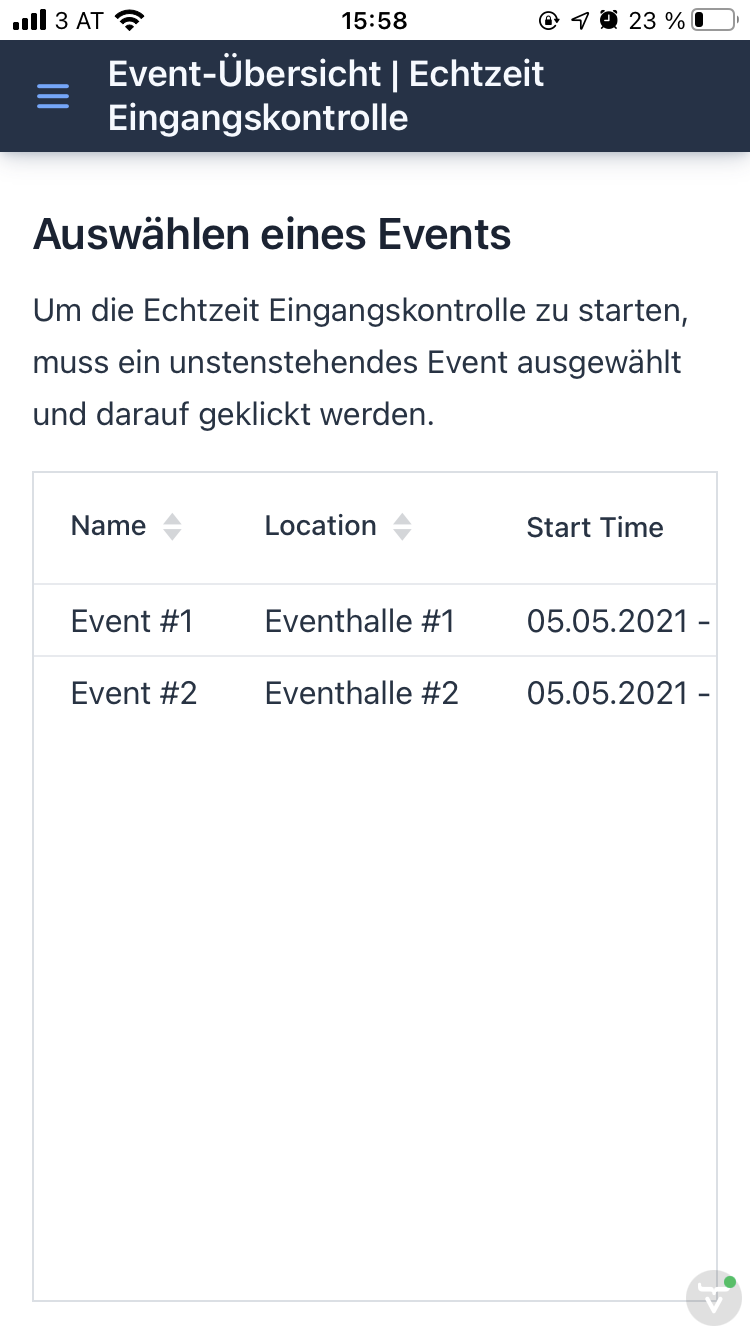
\includegraphics[scale=0.25]{images/Luidold_Results-Vaadin-PWA.png}
    \caption[Die Vaadin Demo als \acs{PWA} unter iOS]{Die Vaadin Demo als \ac{PWA} unter iOS}
    \label{fig:results-vaadin-pwa}
\end{figure}

Weiterführende Funktionalitäten bietet das Vaadin Framework jedoch nur noch eingeschränkt an. Eine Offline-Fähigkeit (die mit dem Kriterium \textit{\nameref{sub-sec:kriterien-datenanbindung}} auf Seite \pageref{sub-sec:kriterien-datenanbindung} zusammenspielt) wird lediglich dahingehend unterstützt, dass eine konfigurierbare Offline-Seite angezeigt wird, sollte die Internetverbindung unterbrochen werden. Das lokale Cachen von Daten oder das Navigieren durch die Anwendung, ohne der Darstellung von Daten, wird nicht unterstützt. Durch diesen Umstand lässt sich die \ac{PWA} ohne Netzwerkverbindung praktisch nicht nutzen und verliert die anderweitig vorhanden Vorteile.

\subsection{\acs{PWA} mit Offline-Fähigkeit bei Angular}
\label{sub-sec:results-pwa-angular}
Während die Konfiguration der \ac{PWA}-Funktionalität bei Angular etwas mehr Zeit als bei Vaadin in Anspruch nimmt, bietet die zur Verfügung gestellte Integration des sogenannten \textit{Service Workers} deutlich mehr Flexibilität bei der Entwicklung und dadurch mehr  Funktionalitäten bei der tatsächlichen Nutzung der Anwendung.

\medskip

Nach dem Ausführen des Befehls \texttt{ng add @angular-pwa} wird von Angular ein Großteil der initialen Konfiguration und Installation aller Abhängigkeiten übernommen. Im Anschluss steht die Webanwendung, gleich wie im vorherigen Abschnitt beschrieben, als Website und installierbare Applikation (sprich \ac{PWA}) zur Verfügung. Abbildung \ref{fig:results-angular-pwa} auf Seite \pageref{fig:results-angular-pwa} zeigt die Angular Demo, ebenfalls wieder auf einem iPhone unter dem Betriebssystem iOS.

\begin{figure}[ht]
    \centering
    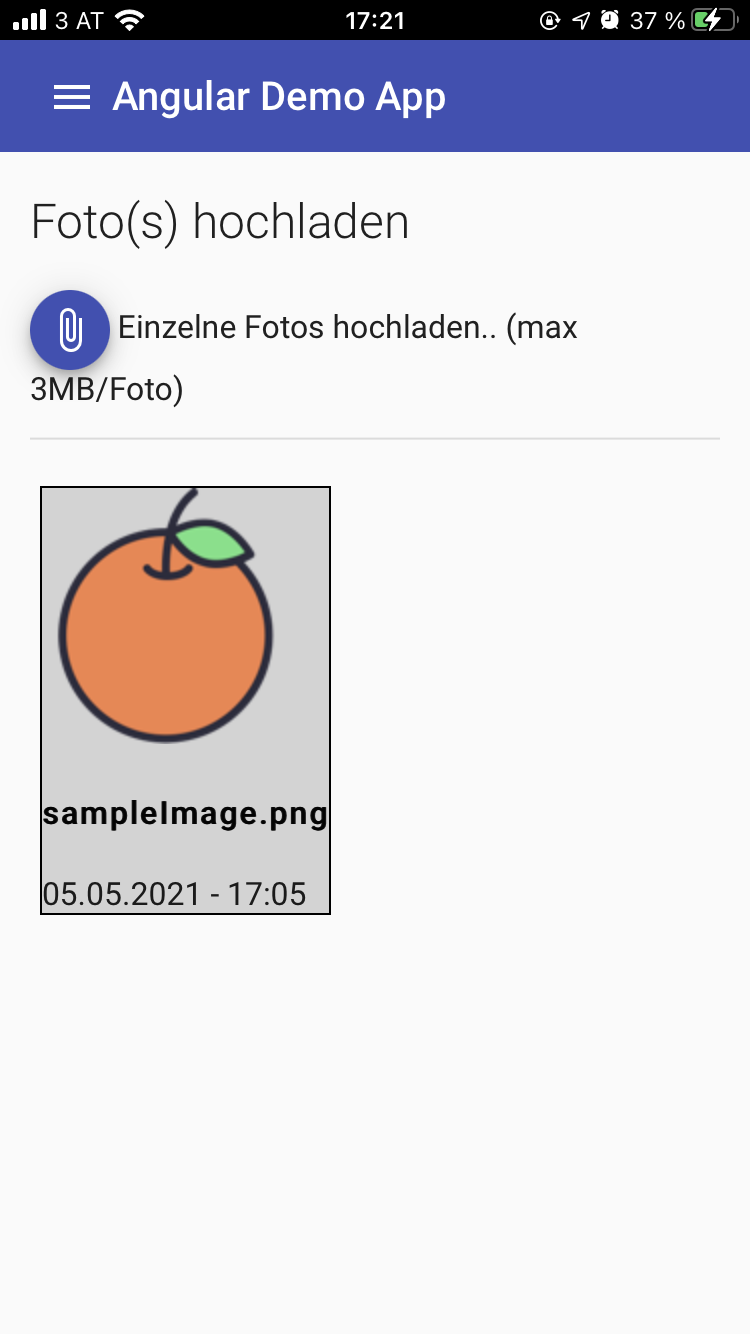
\includegraphics[scale=0.2]{images/Luidold_Results-Angular-PWA.png}
    \caption[Die Angular Demo als \acs{PWA} unter iOS]{Die Angular Demo als \ac{PWA} unter iOS}
    \label{fig:results-angular-pwa}
\end{figure}

Der entscheidende Vorteil des Ansatzes von Angular ist der, dass - neben der Umsetzung als \ac{PWA} selbst - auch mit überschaubarem Aufwand eine Offlinenutzung integriert werden kann. Durch die Installation des \path{@angular-pwa} Package werden verschiedene Konfigurationsdateien für den Service Worker im Projekt hinterlegt. Mit nur wenigen Änderungen an diesen Dateien kann Angular mitgeteilt werden, welche Daten bei einem Aufruf eines API Endpunkts lokal zwischengespeichert beziehungsweise gecached werden sollen. Quellcode \ref{code:results-angular-service-worker} auf Seite \pageref{code:results-angular-service-worker} zeigt die vorgenommen Änderungen an der \path{ngsw-config.json} Datei, welche bewirken, dass die gecacheten Daten der Endpunkte \path{/events}, \path{/attendees} und \path{/photos} verwendet werden sollen, sollte keine aktive Netzwerkverbindung zum Zeitpunkt des Aufrufs der Seite bestehen.

\begin{listing}[ht]
    \renewcommand{\fcolorbox}[4][]{#4}
    \inputminted[fontsize=\footnotesize,linenos,breaklines]{json}{code/Luidold_Results-Angular-ServiceWorker.json}
    \caption[Konfiguration der \ac{PWA} Offline-Funktionalität in der \texttt{ngsw-config.json} Datei]{Konfiguration der \ac{PWA} Offline-Funktionalität in der \texttt{ngsw-config.json} Datei}
    \label{code:results-angular-service-worker}
\end{listing}

Die oben gezeigte Konfiguration ermöglicht es Anwender:innen also, zuvor aufgerufene Daten ansehen zu können, wenn das jeweilige Gerät offline ist. Zudem ermöglicht die Implementierung des Service Workers von Angular die Nutzung der kompletten Anwendung im Offline-Modus. Das bedeutet, dass auch zwischen bestehenden Seiten beziehungsweise Views navigiert werden kann, womit sich die Umsetzung von Angular deutlich von der von Vaadin abhebt.

\section{Wiederverwendbare Komponenten bei beiden Frameworks}
\label{sec:ergebnisse-wiederverwendbarkeit}
Das zweite Kriterium, welches bei der Umsetzung der Demo-Applikationen maßgeblich betrachtet wurde, ist das gezielte Einsetzen von wiederverwendbaren Komponenten (siehe dazu \textit{\nameref{sub-sec:kriterien-web-components}} auf Seite \pageref{sub-sec:kriterien-web-components}). Ähnlich wie bei der Umsetzung der Anwendungen als \ac{PWA}, bieten auch bei diesem Punkt beide Frameworks entsprechende Möglichkeiten, die stellenweise jedoch auf die jeweilige Programmiersprache und die dazugehörigen Programmierparadigmen zurückgeführt werden können.

\subsection{Objektorientierte Komponenten von Vaadin}
\label{sub-sec:results-wiederverwendbarkeit-vaadin}
Vaadin Flow baut auf Java und somit einer objektorientierten Programmiersprache auf. Das bedeutet, dass sowohl die von Vaadin entwickelten Vaadin Components als auch eigene Bestandteile der Anwendung in Java-typischer Weise verwendet und erweitert werden können.

\begin{figure}[ht]
    \centering
    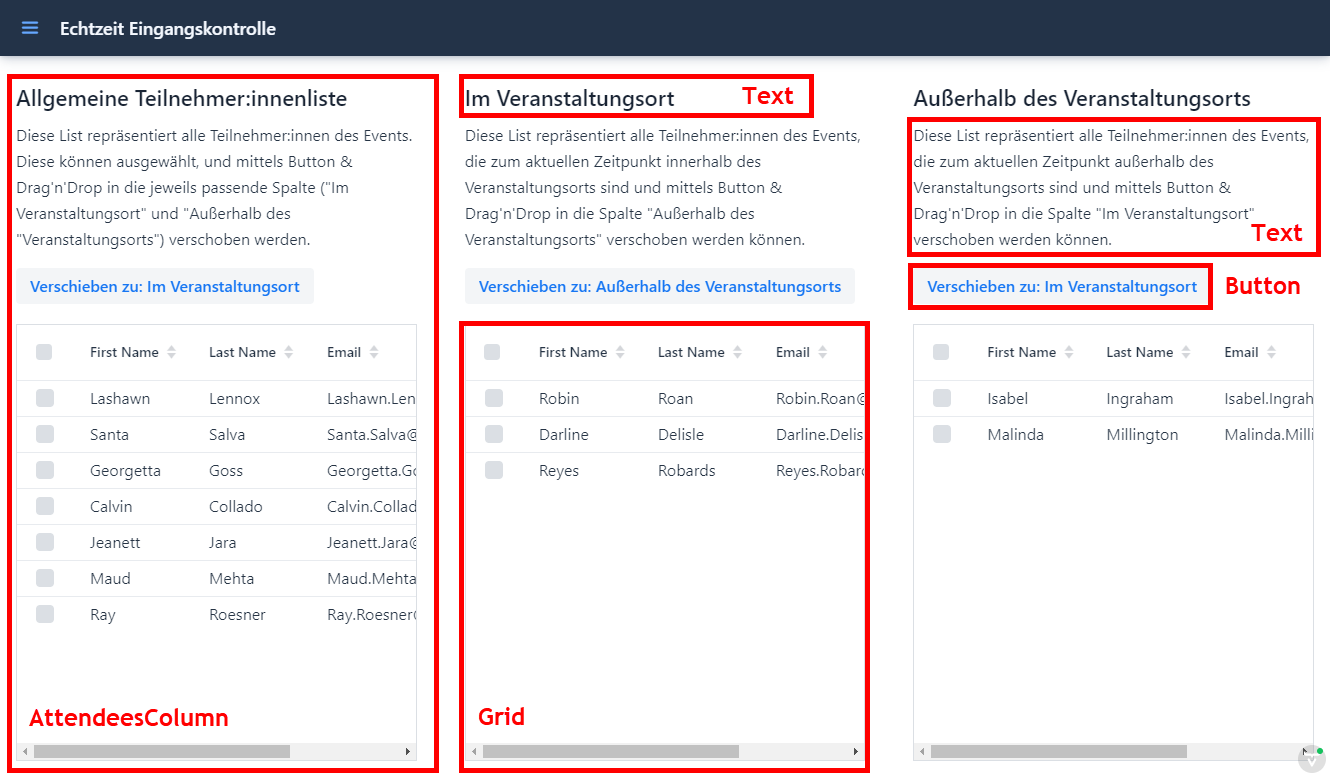
\includegraphics[scale=0.4]{images/Luidold_Results-Vaadin-Components.png}
    \caption[Komponenten der \textit{Echtzeit Eingangskontrolle} bei Vaadin]{Komponenten der \textit{Echtzeit Eingangskontrolle} bei Vaadin}
    \label{fig:results-vaadin-components}
\end{figure}

Ein deutliches Beispiel für die Umsetzung von wiederverwendbaren Komponenten stellt die Übersicht der \textit{Echtzeit Eingangskontrolle} dar. Die in Abbildung \ref{fig:results-vaadin-components} auf Seite \pageref{fig:results-vaadin-components} rot eingerahmten Elemente bilden eigenständige Komponenten ab, die entweder von Vaadin bereitgestellt werden oder im Zuge der Umsetzung eigenständig entwickelt wurden. Diese lassen sich wie folgt einteilen:

\begin{itemize}
    \item \texttt{AttendeesColumn} ist eine Eigenentwicklung und entspricht einer der insgesamt drei dargestellten, großen Spalten. Diese Klasse umfasst die nachfolgend aufgelisteten Komponenten, stellt diese in einem vertikalen Layout dar und dient zur zentralen Konfiguration und zur Übergabe als übergeordnetes \enquote{Element} an die Java API von Vaadin.
    \item \texttt{Grid} ist eine Vaadin Komponente und entspricht einer der drei dargestellten Tabellen. Mittels verschiedener Attribute und Methoden kann die Tabelle beliebig angepasst und ausgetauscht oder bei Bedarf über die gewohnte Klassenhierarchie von Java weiter spezialisiert werden.
    \item \texttt{Text} \& \texttt{Button} sind ebenfalls Vaadin Components und bieten ähnliche Konfigurationsmöglichkeiten wie die \texttt{Grid} Komponente.
\end{itemize}

Aufgrund der von Vaadin vorgegebenen Empfehlungen und Herangehensweisen, enthält eine übergeordnete View-Klasse die oben genannten Bestandteile und die dazugehörige Logik. Quellcode \ref{code:results-vaadin-components} im Anhang auf Seite \pageref{code:results-vaadin-components} zeigt in einem kurzen Ausschnitt, wie solch eine Klasse aufgebaut ist.

\medskip

Die \textit{Vaadin Components} selbst sind bereits eigenständige Web Components, wie in Abschnitt \ref{sub-sec:vaadin-components} ab Seite \pageref{sub-sec:vaadin-components} beschrieben wurde. Für die Umsetzung der einzelnen User Stories hat die Verwendung der bestehenden Vaadin Components sowie die gezielte Entwicklung von einigen, wenigen Klassen ausgereicht, um eine adäquate Wiederverwendbarkeit zu gewährleisten. Sofern Komponenten noch weiter abstrahiert werden müssen, bietet Vaadin jedoch die Möglichkeit\footnote{\href{https://vaadin.com/docs/latest/flow/creating-components/overview}{Creating Components | Vaadin Docs (https://vaadin.com/docs/latest/flow/creating-components/overview)}}, eigene Java Komponenten erstellen zu können.

\subsection{Wiederverwendbare Angular Komponenten}
\label{sub-sec:results-wiederverwendbarkeit-angular}
Im Vergleich zu den vorgefertigten Komponenten, die Vaadin bereitstellt, unterscheidet sich die Herangehensweise von Angular bei diesem Thema. Die Komponenten, die entweder händisch oder mit dem Befehl \texttt{ng g component <name>} erstellt werden können, bestehen jeweils aus einer HTML, einer CSS und einer JavaScript/TypeScript Datei. Quellcode \ref{code:results-angular-components} auf Seite \pageref{code:results-angular-components} zeigt einen Ausschnitt solch einer Komponente und wie diese grundlegend aufgebaut ist.

\begin{listing}[ht]
    \renewcommand{\fcolorbox}[4][]{#4}
    \inputminted[fontsize=\footnotesize,linenos,breaklines]{js}{code/Luidold_Results-Angular-Components-CodeSample.ts}
    \caption[Ausschnitt der \texttt{EntranceControl} Komponente]{Ausschnitt der \texttt{EntranceControl} Komponente}
    \label{code:results-angular-components}
\end{listing}

In Zeile 3-7 ist deutlich zu erkennen, wie die Aufteilung der verschiedenen Technologien funktioniert und in welchen Dateien diese zu finden sind. Um den selbst erstellten und oben als Beispiel aufgeführten Component in der Anwendung einsetzen zu können, wird der HTML-Tag \texttt{<app-entrance-control>} verwendet, der entsprechend an der gewünschten Stelle eingefügt werden muss.

\medskip

Die Aufteilung der Logik fällt bei Angular zudem anders als bei Vaadin aus, da die einzelnen Komponenten vermehrt eigenständig sind und selbst Logik beinhalten. Das liegt primär daran, dass die Komponenten untereinander weitestgehend frei agieren und referenziert werden können. Es gibt zwar einige, übergeordnete Steuerungselemente, diese fallen wegen der fehlenden Klassenhierarchie jedoch stellenweise deutlich weniger ins Gewicht.

\medskip

Das Auftrennen in verschiedene, wiederverwendbare Komponenten fällt am Beispiel der \textit{Echtzeit Eingangskontrolle} dennoch ähnlich wie bei Vaadin aus, wie Abbildung \ref{fig:results-angular-components} auf Seite \pageref{fig:results-angular-components} zeigt. Die benötigten (HTML) Elemente werden dabei in einer HTML-Datei einer Komponente zusammengeführt und passend angeordnet und können dann, samt der zugehörigen Logik und dem Styling, genutzt werden.

Hervorzuheben ist hierbei jedoch, dass die von Angular Material bereitgestellten \textit{UI components} in vielen Fällen ergänzend zu nativen HTML Elementen eingesetzt werden und deren Funktionalität lediglich erweitern, nicht jedoch komplett ersetzen. Als Beispiel dafür kann die in rot eingezeichnete Tabelle herangenommen werden. Diese entspricht einem regulären HTML \texttt{table} Tag, welcher zusätzlich mit Angular Material Attributen versehen wurde (beispielsweise \texttt{mat-table matSort [dataSource]}).

\begin{figure}[ht]
    \centering
    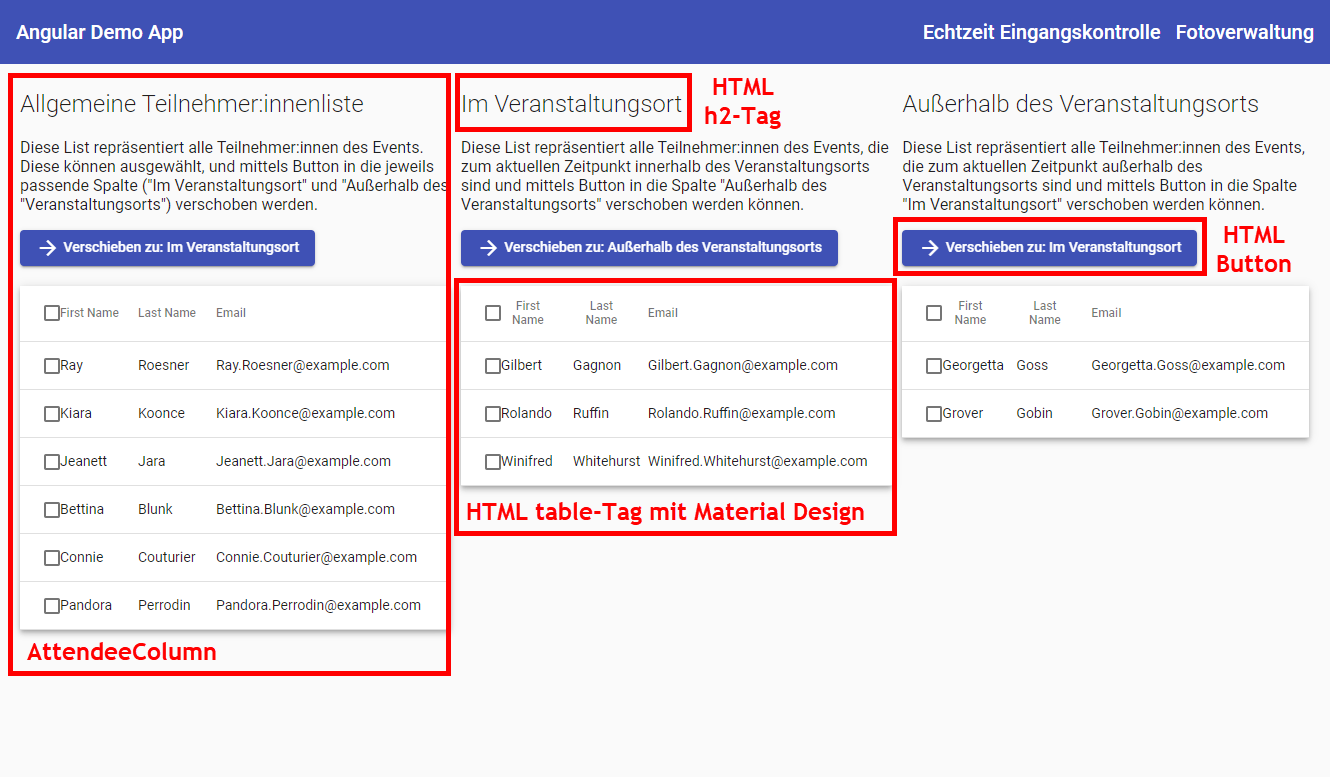
\includegraphics[scale=0.4]{images/Luidold_Results-Angular-Components.png}
    \caption[Komponenten der \textit{Echtzeit Eingangskontrolle} bei Angular]{Komponenten der \textit{Echtzeit Eingangskontrolle} bei Angular}
    \label{fig:results-angular-components}
\end{figure}

Wie bei der Umsetzung der Vaadin Anwendung, wurde auch bei der Entwicklung der Angular Demo auf die Entwicklung von entkoppelten Web Components verzichtet und primär auf Komponenten gesetzt, die im projektspezifische Kontext wiederverwendet werden können. Bei Bedarf bietet jedoch auch Angular die Möglichkeit\footnote{\href{https://angular.io/guide/elements/}{Angular Elements (https://angular.io/guide/elements)}}, abstrahierte Elemente analog zu den Web Component Standards zu entwickeln.

\section{Unterschiede bei der Datenanbindung}
\label{sec:results-datenanbindung}
Neben den zwei bisher behandelten Kriterien wurde speziell auch auf die Thematik der lokalen und externen Datenanbindung beziehungsweise Datenhaltung der Anwendungen geachtet (siehe dazu \textit{\nameref{sub-sec:kriterien-datenanbindung}} auf Seite \pageref{sub-sec:kriterien-datenanbindung}).

Da sich die Technologie-Stacks von Vaadin und Angular deutlich unterscheiden, eröffnen sich in beiden Fällen unterschiedliche Möglichkeiten und Herangehensweisen, wie die jeweiligen Daten der Applikationen gespeichert und Benutzer:innen wieder zur Verfügung gestellt werden können. Die dabei erzielten Ergebnisse unterscheiden sich bisher am deutlichsten voneinander und hatten unterschiedliche Auswirkungen auf die Planung und Entwicklung der Anwendungen.

\subsection{Serverseitige Datenhaltung mittels Java}
\label{sub-sec:result-datenanbindung-vaadin}
Als auf einem Server ausgeführte Programmiersprache bietet Java diverse Vorteile, wenn es um die Anbindung an Datenbanken und persistente Datenspeicher geht. Diese Vorteile stehen während der Entwicklung einer Vaadin Flow Applikation uneingeschränkt zur Verfügung und werden durch das mitgelieferte Spring Boot zusätzlich erleichtert.

\medskip

Während der Entwicklung der Vaadin Demo-Anwendung ist das ORM Framework Hibernate zum Einsatz gekommen. Dieses hat sich, in Zusammenspiel mit Spring Boot, um den Datenzugriff sowie die Verwaltung der eingesetzten \ac{JPA} Entities gekümmert. Für das Persistieren der Daten wurde eine In-Memory \textit{H2}\footnote{\href{https://h2database.com/}{H2 Database Engine (https://h2database.com)}} Datenbank verwendet, welche jedoch mit minimalem Aufwand gegen ein beliebiges Datenbankmanagementsystem ausgetauscht werden kann.

\medskip

Da Vaadin Flow sowohl die \ac{UI} als auch die Anwendungslogik in einem Programmcode vereint, können die im Browser angezeigten Daten direkt und ohne zusätzlich Austausch in der weiteren Ablauflogik verwendet werden. Quellcode \ref{code:results-vaadin-datenanbindung} auf Seite \pageref{code:results-vaadin-datenanbindung} zeigt ein Beispiel, wie von Benutzer:innen zur Verfügung gestellte Daten (in diesem Fall ein Foto in Form eines Datenstreams in Zeile 4) direkt genutzt werden können, um in einer Datenbank gespeichert zu werden.

\begin{listing}[ht]
    \inputminted[fontsize=\footnotesize,linenos,breaklines]{java}{code/Luidold_Results-Vaadin-Datenanbindung-CodeSample.java}
    \caption[Beispiel für das direkte Verwenden von Daten aus der \ac{UI} in Vaadin]{Beispiel für das direkte Verwenden von Daten aus der \ac{UI} in Vaadin}
    \label{code:results-vaadin-datenanbindung}
\end{listing}

Ähnlich einfach gestaltet sich der Zugriff auf gespeicherte Daten, die nach einem Zugriff auf die Datenbank ebenfalls im normalen Ablauf des Java Programmcodes genutzt und schlussendlich den Anwender:innen direkt angezeigt werden können. Wo sich Vaadin Flow hingegen weniger flexibel zeigt, ist beim lokalen Speichern von Daten direkt im Browser. Zwar gibt es die Möglichkeit, den Komponenten JavaScript in Textform zu übergeben und dieses dann im Browser ausführen zu lassen, ein direkter Zugriff ohne JavaScript Kenntnisse ist jedoch, zumindest zum aktuellen Stand dieser Arbeit, nicht möglich.

\subsection{Externes Backend zur Datenspeicherung für Angular}
\label{sub-sec:result-datenanbindung-angular}
Vaadin bietet mit der zugrundeliegenden Programmiersprache Java diverse Herangehensweisen, wie eine Datenanbindung umgesetzt werden kann. Bei Angular hingegen gibt es standardmäßig keine solch eine Möglichkeit, wenn die Daten zentral auf einem Server statt lokal im Webbrowser gespeichert werden sollen.

\medskip

Wie in Abschnitt \ref{sub-sub-sec:kommunikation-herangehensweise-angular} auf Seite \pageref{sub-sub-sec:kommunikation-herangehensweise-angular} beschrieben, ermöglicht Angular eine weitestgehend freie und anpassbare Kommunikation mit einem beliebigen Backend beziehungsweise Server. Im Zuge der Umsetzung der Angular Demo-Applikation wurde daher, neben der eigentlichen Angular Anwendung selbst, ein eigenständiges Backend entwickelt, welches die externe Speicherung der Daten übernimmt. Das auf Node.js und Express basierende Backend ist hauptsächlich für das Speichern und Abrufen der Daten verantwortlich und setzt das mit einer reinen In-Memory Lösung um.

Quellcode \ref{code:results-angular-datenanbindung} auf Seite \pageref{code:results-angular-datenanbindung} zeigt beispielhaft die Kommunikation mit dem \path{/events} API Endpunkt auf. Wie hierbei ersichtlich wird, spielt es für Angular selbst keine Rolle, von wo genau die Daten stammen beziehungsweise auf welche Weise diese erstellt wurden, solange sie in einem kompatiblen Format (beispielsweise \acs{JSON}) übermittelt werden.

\begin{listing}[ht]
    \renewcommand{\fcolorbox}[4][]{#4}
    \inputminted[fontsize=\footnotesize,linenos,breaklines]{js}{code/Luidold_Results-Angular-Datenanbindung-CodeSample.ts}
    \caption[Beispielhafter Auszug der Kommunikation mit dem Backend bei Angular]{Beispielhafter Auszug der Kommunikation mit dem Backend bei Angular}
    \label{code:results-angular-datenanbindung}
\end{listing}

Deutliche Vorteile bietet Angular, beziehungsweise JavaScript und Type-Script selbst, beim Zugriff auf den lokalen Speicher direkt im Browser. Sowohl \textit{Cookies} als auch der \textit{SessionStorage} und \textit{LocalStorage} können in der gesamten Applikation verwendet werden, um Daten auf dem jeweiligen Endgerät (zwischen) zu speichern. Genutzt wurde diese Möglichkeit für die Offlinenutzung der Fotoverwaltung (siehe dazu \textit{\nameref{sub-sub-sec:user-story-2}} auf Seite \ref{sub-sub-sec:user-story-2}), bei der Fotos \texttt{base64} encoded im LocalStorage abgelegt wurden, bis wieder eine aktive Internetverbindung besteht. Etwaige Limitierungen bezüglich der maximalen Speichergröße oder ähnlichem werden von Angular nicht vorgenommen und hängen daher in der Regel vom jeweiligen Betriebssystem und Webbrowser selbst ab.

\section{Anderweitige Ergebnisse der Umsetzung der User Stories}
\label{sec:results-user-stories}
Neben den bisher behandelten Punkten, die größtenteils auf die vorab definierten Kriterien bezogen sind, haben sich bei der Umsetzung der Demo-Applikationen zusätzlich einige weitere Erkenntnisse ergeben, die im Folgenden kurz aufgezeigt werden.

\subsection{Umsetzung der Echtzeit-Funktionalität}
\label{sub-sec:results-user-stories-echtzeit}
Die bei \textit{\nameref{sub-sub-sec:user-story-1}} geforderte Echtzeit-Funktionalität wurde in beiden Anwendungen umgesetzt und funktioniert für Anwender:innen der Applikationen identisch. Die technische Umsetzung und der damit verbundene Aufwand unterscheiden sich hierbei jedoch von einander.

\medskip

Vaadin ermöglicht mit der Konfiguration von \textit{Server Push}\footnote{\href{https://vaadin.com/docs/latest/flow/advanced/server-push}{Server Push | Vaadin Docs (https://vaadin.com/docs/latest/flow/advanced/server-push)}} das Aktualisieren der \ac{UI} vom Server aus, ohne dass Benutzer:innen manuell eine Aktualisierung anfordern müssen. Benötigt wird dafür die \texttt{@Push} Annotation sowie eine Klasse, welche das Verwalten der unterschiedlichen Clients übernimmt und der Ablauflogik erlaubt, Aktualisierungen auszulösen, sobald bestimmte Kriterien erfüllt wurden. Die tatsächlichen Änderungen auf den Clients übernimmt Vaadin dabei wieder automatisch und erfordert keine manuell ausgeführte Kommunikation mit dem jeweiligen Frontend.

\medskip

Um Daten in Echtzeit ändern und aktualisieren zu können, bedarf es einer fortlaufenden Verbindung vom Backend zum Frontend. Da Angular dies von Haus aus nicht selbst unterstützt, wurde die Funktionalität mittels \textit{Socket.IO}\footnote{\href{https://socket.io/}{Socket.IO (https://socket.io)}} in das Node.js Backend integriert und in die Angular Anwendung eingebunden. Die in Quellcode \ref{code:results-angular-echtzeit} auf Seite \pageref{code:results-angular-echtzeit} demonstrierte Verbindung wird mit \textit{WebSockets} aufgebaut und ermöglicht das bidirektionale Senden und Empfangen von Daten, ohne dass die Änderungen auf dem Client von einem:einer Anwender:in angefordert werden müssen.

\begin{listing}[ht]
    \inputminted[fontsize=\footnotesize,linenos,breaklines]{js}{code/Luidold_Results-Angular-Echtzeit-CodeSample.ts}
    \caption[Echtzeitkommunikation mittels WebSockets bei Angular]{Echtzeitkommunikation mittels WebSockets bei Angular}
    \label{code:results-angular-echtzeit}
\end{listing}

\subsection{Implementierung von \enquote{Drag and Drop}}
\label{sub-sec:results-user-stories-drag-drop}
Im Zuge der Umsetzung der \textit{Echtzeit Eingangskontrolle} wurde bei der Vaadin Demo-Applikation die Möglichkeit implementiert, Teilnehmer:innen per \enquote{Drag and Drop} in die passende Spalte verschieben zu können. Die zugrundeliegende Funktionalität wird dabei von Vaadin Flow zur Verfügung gestellt und mittels diverser Listener umgesetzt. Als weiterführende Hilfestellung stellt Vaadin eine ausführliche Dokumentation bereit, wie Drag and Drop bei einer \texttt{Grid} Komponente (entspricht einer Tabelle) umgesetzt werden kann.

\medskip

Bei der Entwicklung der Angular Anwendung wurde ebenfalls versucht, dieselbe Drag and Drop Funktionalität umzusetzen. Zwar bietet Angular mit dem \path{@angular/cdk/drag-drop} Modul eine umfangreiche Möglichkeit, das Verhalten von verschiedenen Elementen dahingehend zu verändern. In Zusammenspiel mit dem HTML \texttt{table} Tag, der verwendeten Datenstruktur und der Anforderung der Echtzeitkommunikation hat die Umsetzung jedoch nicht die gewünschten Resultate erzielt und wurde schlussendlich nicht umgesetzt.

\chapter{Zusammenfassung und Ausblick}
\label{chap:zusammenfassung-ausblick}
TODO

% Literaturverzeichnis:
\clearpage
\phantomsection
\addcontentsline{toc}{chapter}{Literaturverzeichnis}
\printbibliography

% Anhang:
\appendix

\chapter*{Anhang - EntranceControlView Klasse}
\addcontentsline{toc}{chapter}{Anhang - EntranceControlView Klasse}
\label{appendix:entrance-control-view-class}
\begin{listing}[H]
    \inputminted[fontsize=\footnotesize,linenos,breaklines]{java}{code/Luidold_Results-Vaadin-Components-CodeSample.java}
    \caption[Ausschnitt der \texttt{EntranceControlView} Klasse, der einen Teil der Komponentenkonfiguration aufzeigt]{Ausschnitt der \texttt{EntranceControlView} Klasse, der einen Teil der Komponentenkonfiguration aufzeigt}
    \label{code:results-vaadin-components}
\end{listing}

\chapter*{Eidesstattliche Erklärung}
\addcontentsline{toc}{chapter}{Eidesstattliche Erklärung}
Ich erkläre hiermit an Eides statt, dass ich die vorliegende Bachelorarbeit II selbstständig und ohne Benutzung anderer als der angegebenen Hilfsmittel angefertigt habe. Die aus fremden Quellen direkt oder indirekt übernommenen Stellen sind als solche kenntlich gemacht. Die Arbeit wurde bisher weder in gleicher noch in ähnlicher Form einer anderen Prüfungsbehörde vorgelegt und auch noch nicht veröffentlicht.

\vspace{5cm}
\noindent
Dornbirn, am 20. Mai 2021\hfill Dominic Luidold

\end{document}
